\documentclass[12pt]{article}
\usepackage[spanish]{babel}
\usepackage[a4paper, margin=2.5cm]{geometry}
\usepackage[utf8x]{inputenc}
\usepackage{amsmath}
\usepackage{mathptmx}
\renewcommand\spanishtablename{Tabla}
\usepackage[11pt]{moresize}
\usepackage{csvsimple}
\usepackage[table,xcdraw,dvipsnames]{xcolor}
\usepackage{booktabs}
\usepackage{amsfonts}
\usepackage{fancyhdr}
\usepackage[T1]{fontenc}
\usepackage{blindtext}
\usepackage{hyperref}
\usepackage{graphicx}
\usepackage{array, multirow}
\usepackage{gensymb}
\usepackage[nottoc]{tocbibind}
\usepackage{wrapfig}
\usepackage{multicol}
\usepackage[makeroom]{cancel}
\usepackage{subcaption}
\usepackage[OPTIONS]{caption}
\usepackage{booktabs}
\usepackage{float}   
\captionsetup{justification=centerlast,labelfont=bf,textfont=it,font=small}
\setlength{\parindent}{2em}
\addto\captionsspanish{
\renewcommand\contentsname{Índice de Contenidos}
}

\pagestyle{fancy}
\fancyhf{}
\rhead{Universidad Técnica Federico Santa María}
\lhead{Departamento de Mecánica}
\rfoot{Página \thepage}
\renewcommand{\headrulewidth}{1pt}
\renewcommand{\footrulewidth}{1pt}

\begin{document}
\begin{titlepage}
\begin{figure}
    \centering
    
\includegraphics[width=1\textwidth]{logo.png}
\end{figure}

\begin{center}
\vspace*{3cm}
\color{gray}
{\Huge \textbf{Informe de}}\\[0.2cm]
{\Huge \textbf{EVALUACIÓN DOCENTE}}\\[0.2cm]
\color{black}
{\Large{Comité de Desarrollo Curricular}}\\[0.2cm]
{\Large Departamento de Ingeniería Mecánica}\\[0.2cm]
{\Large Primer Semestre del 2018}\\[2.5cm]

\begin{table}[H]
\centering
\begin{tabular}{lll}
{\large ELABORACIÓN: } & {\large Profesor:} & {\large Guillermo González Baquedano} \\
 & {\large Ayudante:} & {\large Paz Aranibar Sanchez}
\end{tabular}
\end{table}

\vspace{2cm}
Valparaíso, Agosto del 2019
\end{center}
\end{titlepage}

\newpage
\tableofcontents

\newpage



%%%%%%%%%%%%%% 1. INTRODUCCION Y OBJETIVOS%%%%%%%%%%%%%%
\section{Introducción y Objetivos.}
\begin{text}
En el presente informe se entregan los principales resultados del proceso de evaluación docente, correspondiente al Primer Semestre del año 2018, realizado por el Comité de Desarrollo Curricular del Departamento de Ingenieria Mecánica (DIMEC). El primordial objetivo de este informe, según el artículo N° 43 del Reglamento del DIMEC, es realizar un análisis y evaluación de cada asignatura impartida por el Departamento, en base a los resultados de la encuesta docente contestada por los alumnos en el sistema SIGA (www.siga.utfsm.cl) y las Actas de Notas durante el semestre correspondiente.
\end{text}



%%%%%%%%%%%%%%%%%%% 2. Antecedentes de la act del DIMEC en el 2017-2  %%%%%%%%%%%%%%%%

\section{Antecedentes de la actividad docente del departamento de Ingeniería Mecánica el Primer Semestre del 2018.}
\begin{text}
En este apartado se entrega información recopilada por el Comité sobre la muestra considerada para realizar el análisis de la evaluación del presenta informe. 
\par
%%%%%%%%%%%%%%%%%%   2.1 DESCRIPCION DE LA MUESTRA            %%%%%%%%%%%%
\subsection{Descripción de la Muestra}
Se consideran las asignaturas impartidas en el período y que son de responsabilidad del DIMEC (Diurna, Campus Casa Central y Campus Santiago). En total son: 
\end{text}
\begin{itemize}
    \item 108 paralelos: 62 en Campus Casa Central y 46 en Campus Santiago.
    \item 44 asignaturas impartidas por 55 profesores,
    \item 3153 inscripciones en sus cursos (1816 en Campus Casa Central y 1337 en Campus Santiago).
    \item 26 profesores de jornada completa impartieron 53 paralelos de asignaturas.
    \item 29 profesores de jornada parcial impartieron 62 paralelos de asignaturas.
\end{itemize}
\begin{text}
\indent 
En Campus Casa Central, de un total de 62 paralelos, 45 de ellos son destinados exclusivamente para las carreras del DIMEC (Ingeniería Civil Mecánica o ICM e Ingeniería Mecánica Industrial o IMI), 6 paralelos para las carreras de DIMEC en conjunto con otras carreras y 11 paralelos están destinados solo para carreras de otros departamentos. \par
En total, los paralelos destinados para cada carrera son:
\end{text}
\begin{itemize}
    \item 45 paralelos exclusivos para carreras DIMEC. 
    \item 4 paralelos para carreras DIMEC, Ingeniería Civil Eléctrica e Ingeniería Eléctrica.
    \ITEM 2 paralelos para carreras DIMEC en conjunto con Ingeniería Civil Industrial.
    \item 4 paralelos para Ingeniería Civil Industrial.  
    \item 1 paralelos para Ingeniería Civil Industrial en régimen vespertino.
    \item 1 paralelos para Ingeniería en Diseño de Productos. 
    \item 2 paralelos para Ingeniería Civil Química.
    \item 3 paralelo para Ingeniería Civil Industrial e Ingeniería en Diseño de Productos.
\end{itemize}
\vspace{10mm}
\begin{text}
\indent
En Campus Santiago, de un total de 46 paralelos, 31 de ellos son destinados exclusivamente para las carreras del DIMEC (Ingeniería Civil Mecánica), 3 paralelos para Ingeniería Civil Mecánica en conjunto con otras carreras y 12 paralelos están destinados solo para carreras de otros departamentos.\par
En total, los paralelos destinados para cada carrera son:
\end{text}
\begin{itemize}
    \item 31 paralelos para Ingeniería Civil Mecánica.
    \item 3 paralelos para Ingeniería Civil Mecánica e Ingeniería Civil Eléctrica.
    \item 7 paralelos para Ingeniería Civil Industrial.
    \item 4 paralelos para Ingeniería Civil Química. 
    \item 1 paralelo para Ingeniería Civil.
\end{itemize}
\begin{text}
\indent
Cabe mencionar que no se han considerado en este análisis las asignaturas correspondientes a los últimos semestres cuyo número de alumnos fuese reducido. Estas son: Investigación Aplicada II (ICM-392), Trabajo de Título en Ingeniería Civil Mecánica (MEC-399) y Trabajo de Título en Ingeniería Mecánica Industrial (MEC-398). Tampoco se consideran las asignaturas con inscripciones menores a cinco alumnos.
\end{text}


%%%%%%%%%%%%%%  2.2 DESCRIPCION DE LA ENCUESTA         %%%%%%%%%%%
\subsection{Descripción de la Encuesta} \label{2.2}
\begin{text}
En cuanto a la encuesta docente aplicada en la UTFSM el periodo 2018-1, esta está basada en los factores presentados a continuación:
\end{text}

\begin{table}[H]
\centering
\resizebox{.9\textwidth}{!}{
\begin{tabular}{|l|l|}
\hline
\rowcolor[HTML]{DAE8FC} 
\multicolumn{1}{|c|}{\cellcolor[HTML]{DAE8FC}\textbf{N°}} & \multicolumn{1}{c|}{\cellcolor[HTML]{DAE8FC}\textbf{Pregunta}} \\ \hline
1 & Cumplió con las actividades planificadas para el curso \\ \hline
2 & Asistió a clases con regularidad \\ \hline
3 & Asistió a clases con puntualidad \\ \hline
4 & Distribuyó correctamente el tiempo del curso \\ \hline
5 & Utilizó criterios de evaluación claros y explícitos \\ \hline
6 & Aplicó evaluaciones que se ajustaron a las actividades desarrolladas en el curso \\ \hline
7 & Entregó las calificaciones en los plazos establecidos \\ \hline
8 & Mostró dominio de los contenidos del curso \\ \hline
9 & Transmitió los contenidos del curso de forma clara y comprensible \\ \hline
10 & Creó un ambiente favorable para el aprendizaje \\ \hline
11 & Mostró preparación de las clases \\ \hline
12 & Respondió adecuadamente las preguntas de los estudiantes \\ \hline
13 & Motivó a los estudiantes a adquirir el contenido del curso \\ \hline
14 & Estimuló la participación activa de los estudiantes en sus clases \\ \hline
15 & Promovió el diálogo entre los estudiantes \\ \hline
16 & Fue respetuoso con los estudiantes \\ \hline
17 & Estuvo abierto a recibir críticas y sugerencias de parte de los estudiantes \\ \hline
18 & Estableció una relación de confianza con los estudiantes \\ \hline
19 & Mostró compromiso con el proceso de aprendizaje de los estudiantes \\ \hline
\end{tabular}}
\caption{Factores evaluados en la Encuesta Docente 2017-2.}
\end{table}

\begin{text}
Cabe destacar que esta encuesta está enfocada solamente a la actuación del profesor asociada al modelo educativo, no contempla los otros aspectos como: ayudantías, laboratorios y participación del estudiante.\par
Se presenta el resumen de actuación del profesor, que considera agrupación de estos ítems y su ponderación en la evaluación global:
\end{text}

\begin{equation}
    \textbf{\textit{Evaluación global}} = 0,5CH + 0,3R + 0,2F
    \label{equation:ecuacionEG}
\end{equation}

\begin{table}[H]
\resizebox{\textwidth}{!}{
\begin{tabular}{lll}
Donde: &                                                 &                                               \\
CH     & Manejo del contenido y Habilidades pedagógicas. & Promedio Factores: 8, 9, 10, 12, 13, 14 y 19. \\
R      & Relación profesor/estudiante.                   & Promedio Factores: 15, 16, 17 y 18.           \\
F      & Aspectos formales.                              & Promedio Factores: 1, 2, 3, 4, 5, 6, 7 y 11. 
\end{tabular}}
\end{table}


\begin{text}
La escala de calificación es de 1 a 4, donde 1 corresponde a una valoración de Nunca o Casi Nunca, 2 a A Veces, 3 a Frecuentemente y 4 a Siempre. 
\par
Los resultados obtenidos en la encuesta de evaluación docente realizada vía SIGA para el primer semestre del 2018 serán presentados según los siguientes cuatro aspectos señalados:
\end{text}
\begin{itemize}
    \item Evaluación global
    \item Manejo de contenido y habilidades pedagógicas.
    \item Relación profesor/estudiante.
    \item Aspectos formales.
\end{itemize}


\subsection{Tablas de Información}
\begin{text}
En las Tablas \ref{table:resumenCC} y \ref{table:resumenCS} que se presentan a continuación se enlistan las asignaturas dictadas por el DIMEC durante el primer semestre del año 2018, separadas entre las impartidas en Campus Casa Central y Campus Santiago (San Joaquín y Vitacura), respectivamente.
\par
Cada tabla está compuesta por los siguientes items: sigla de la asignatura (\textbf{Sigla}), el nombre de la asignatura (\textbf{Asignatura}), el número de paralelo (\textbf{Par.}), el número de alumnos inscrítos en la asignatura (\textbf{Insc.}), el porcentaje de éstos que respondió la encuesta docente (\textbf{\% Res.}), el promedio de notas de la asignatura (\textbf{Prom.}) y el porcentaje de alumnos que aprobó el ramo (\textbf{\% Apr.}).
\par
Estas tablas se obtuvieron a partir de la información de las encuestas docentes y de la información de aprobación de cada asignatura disponibles en el sistema SIGA. 
\par
\end{text}

\begin{table}[H]
\resizebox{\textwidth}{!}{
\begin{tabular}{|c|l|c|c|c|c|c|}
\hline
\rowcolor[HTML]{91C1EE} 
\textbf{Sigla} & \multicolumn{1}{c|}{\cellcolor[HTML]{91C1EE}\textbf{Asignatura}} & \textbf{Par} & \textbf{Insc.} & \textbf{\%Resp.} & \textbf{Prom.} & \textbf{\%Aprob.} \\ \hline
\rowcolor[HTML]{DAEBFB} 
ICM256 & ANALISIS DE ESFUERZOS & 1 & 24 & 62,50 & 70,75 & 100,00 \\ \hline
\rowcolor[HTML]{DAEBFB} 
ICM286 & FUNDAMENTOS DEL DISEÑO & 1 & 41 & 48,78 & 65,73 & 95,12 \\ \hline
\rowcolor[HTML]{DAEBFB} 
ICM312 & TECNOLOGIA DE LA COMBUSTION & 1 & 23 & 65,22 & 66,74 & 100,00 \\ \hline
\rowcolor[HTML]{DAEBFB} 
ICM363 & AUTOMATIZACION & 1 & 16 & 25,00 & 75,25 & 93,75 \\ \hline
\rowcolor[HTML]{DAEBFB} 
ICM363 & AUTOMATIZACION & 2 & 12 & 66,67 & 69,83 & 100,00 \\ \hline
\rowcolor[HTML]{DAEBFB} 
ICM370 & GESTION Y CONTROL DE OPERA. LOGISTICAS & 1 & 38 & 57,89 & 81,03 & 100,00 \\ \hline
\rowcolor[HTML]{DAEBFB} 
ICM382 & PROYECTOS EN INGENIERIA MECANICA & 1 & 24 & 62,50 & 85,33 & 100,00 \\ \hline
\rowcolor[HTML]{DAEBFB} 
ICM382 & PROYECTOS EN INGENIERIA MECANICA & 2 & 30 & 73,33 & 82,40 & 100,00 \\ \hline
\rowcolor[HTML]{DAEBFB} 
ICM382 & PROYECTOS EN INGENIERIA MECANICA & 3 & 34 & 44,12 & 79,82 & 100,00 \\ \hline
\rowcolor[HTML]{DAEBFB} 
ILM152 & ELEMENTOS DE MECANICA Y RESISTENCIA DE MAT. & 2 & 57 & 80,70 & 57,28 & 78,95 \\ \hline
\rowcolor[HTML]{DAEBFB} 
ILM212 & TERMODINAMICA II & 1 & 70 & 77,14 & 74,01 & 97,14 \\ \hline
\rowcolor[HTML]{DAEBFB} 
ILM254 & MECANICA DE MAQUINAS & 1 & 25 & 52,00 & 65,60 & 72,00 \\ \hline
\rowcolor[HTML]{DAEBFB} 
ILM286 & FUNDAMENTOS DE DISEÑO & 1 & 28 & 71,43 & 78,82 & 100,00 \\ \hline
\rowcolor[HTML]{DAEBFB} 
ILM286 & FUNDAMENTOS DE DISEÑO & 2 & 31 & 70,97 & 82,39 & 100,00 \\ \hline
\rowcolor[HTML]{DAEBFB} 
ILM310 & MOTORES DE COMBUSTION INTERNA & 1 & 46 & 56,52 & 69,33 & 95,65 \\ \hline
\rowcolor[HTML]{DAEBFB} 
ILM322 & TURBOMAQUINAS & 1 & 50 & 74,00 & 81,72 & 98,00 \\ \hline
\rowcolor[HTML]{DAEBFB} 
IMM210 & MAQUINAS TERMICAS & 1 & 45 & 53,33 & 73,78 & 97,78 \\ \hline
\rowcolor[HTML]{DAEBFB} 
IMM222 & TURBOMAQUINAS Y PLANTAS DE FUERZA & 1 & 29 & 51,72 & 71,90 & 96,55 \\ \hline
\rowcolor[HTML]{DAEBFB} 
IMM240 & MANTENCION INDUSTRIAL & 1 & 26 & 46,15 & 72,96 & 100,00 \\ \hline
\rowcolor[HTML]{DAEBFB} 
IMM260 & MANDOS Y CONTROL & 1 & 17 & 47,06 & 65,82 & 100,00 \\ \hline
\rowcolor[HTML]{DAEBFB} 
IMM260 & MANDOS Y CONTROL & 2 & 11 & 81,82 & 70,09 & 100,00 \\ \hline
\rowcolor[HTML]{DAEBFB} 
IMM271 & CALIDAD E INGENIERIA & 1 & 22 & 50,00 & 65,26 & 95,83 \\ \hline
\rowcolor[HTML]{DAEBFB} 
IMM284 & MANEJO DE MATERIALES & 1 & 44 & 65,91 & 69,41 & 97,73 \\ \hline
\rowcolor[HTML]{DAEBFB} 
IPM456 & METODO DE ELEMENTOS FINITOS & 1 & 11 & 36,36 & 83,45 & 100,00 \\ \hline
\rowcolor[HTML]{DAEBFB} 
IPM468 & DINAMICA DE FLUIDOS COMPUTACIONAL & 1 & 9 & 0,00 & 74,33 & 100,00 \\ \hline
\rowcolor[HTML]{DAEBFB} 
IWM151 & MECANICA GENERAL & 1 & 49 & 73,47 & 58,61 & 67,35 \\ \hline
\rowcolor[HTML]{DAEBFB} 
IWM160 & MEDICIONES MECANICAS GENERALES & 1 & 24 & 62,50 & 66,88 & 95,83 \\ \hline
\rowcolor[HTML]{DAEBFB} 
IWM160 & MEDICIONES MECANICAS GENERALES & 2 & 24 & 62,50 & 61,25 & 95,83 \\ \hline
\rowcolor[HTML]{DAEBFB} 
IWM175 & TALLER II & 1 & 26 & 65,38 & 66,62 & 88,46 \\ \hline
\rowcolor[HTML]{DAEBFB} 
IWM175 & TALLER II & 2 & 10 & 60,00 & 69,30 & 100,00 \\ \hline
\rowcolor[HTML]{DAEBFB} 
IWM179 & DIBUJO Y TALLER MECANICO & 1 & 15 & 66,67 & 70,93 & 100,00 \\ \hline
\rowcolor[HTML]{DAEBFB} 
IWM185 & GRAFICA EN INGENIERIA & 1 & 40 & 52,50 & 75,45 & 92,50 \\ \hline
\rowcolor[HTML]{DAEBFB} 
IWM185 & GRAFICA EN INGENIERIA & 2 & 22 & 50,00 & 71,50 & 95,45 \\ \hline
\rowcolor[HTML]{DAEBFB} 
IWM185 & GRAFICA EN INGENIERIA & 3 & 38 & 71,05 & 70,00 & 97,37 \\ \hline
\rowcolor[HTML]{DAEBFB} 
IWM187 & GRAFICA DE SISTEMAS MECANICOS & 2 & 14 & 85,71 & 63,86 & 100,00 \\ \hline
\rowcolor[HTML]{DAEBFB} 
IWM210 & TERMODINAMICA GENERAL Y LABORATORIO & 1 & 41 & 80,49 & 59,12 & 80,49 \\ \hline
\rowcolor[HTML]{DAEBFB} 
IWM210 & TERMODINAMICA GENERAL Y LABORATORIO & 2 & 33 & 63,64 & 58,88 & 75,76 \\ \hline
\rowcolor[HTML]{DAEBFB} 
IWM210 & TERMODINAMICA GENERAL Y LABORATORIO & 3 & 47 & 68,09 & 52,57 & 63,83 \\ \hline
\rowcolor[HTML]{DAEBFB} 
IWM220 & MECANICA DE FLUIDOS GENERAL & 1 & 55 & 72,73 & 66,65 & 98,18 \\ \hline
\rowcolor[HTML]{DAEBFB} 
IWM220 & MECANICA DE FLUIDOS GENERAL & 2 & 12 & 58,33 & 73,25 & 91,67 \\ \hline
\rowcolor[HTML]{DAEBFB} 
IWM230 & TRANSFERENCIA DE CALOR & 1 & 50 & 68,00 & 65,92 & 80,00 \\ \hline
\rowcolor[HTML]{DAEBFB} 
IWM230 & TRANSFERENCIA DE CALOR & 2 & 14 & 57,14 & 69,36 & 92,86 \\ \hline
\rowcolor[HTML]{DAEBFB} 
IWM255 & RESISTENCIA DE MATERIALES GENERALES & 1 & 29 & 68,97 & 53,59 & 72,41 \\ \hline
\rowcolor[HTML]{DAEBFB} 
IWM255 & RESISTENCIA DE MATERIALES GENERALES & 2 & 11 & 72,73 & 59,00 & 54,55 \\ \hline
\rowcolor[HTML]{DAEBFB} 
IWM271 & FUNDAMENTOS DE CALIDAD & 1 & 40 & 55,00 & 62,34 & 92,68 \\ \hline
\rowcolor[HTML]{DAEBFB} 
IWM280 & ELEMENTOS DE MAQUINAS & 1 & 52 & 67,31 & 64,29 & 92,31 \\ \hline
\rowcolor[HTML]{DAEBFB} 
IWM320 & GESTION AMBIENTAL & 2 & 62 & 50,00 & 62,69 & 87,10 \\ \hline
\rowcolor[HTML]{DAEBFB} 
IWM371 & SISTEMATIZACION DE LA PRODUCCION & 1 & 45 & 53,33 & 53,69 & 75,56 \\ \hline
\rowcolor[HTML]{DAEBFB} 
MEC119 & FUNDAMENTOS DE CALOR Y FLUIDOS & 1 & 20 & 75,00 & 61,55 & 85,00 \\ \hline
\rowcolor[HTML]{DAEBFB} 
MEC141 & GRÁFICA EN INGENIERÍA MECÁNICA & 1 & 35 & 94,29 & 75,00 & 97,14 \\ \hline
\rowcolor[HTML]{DAEBFB} 
MEC141 & GRÁFICA EN INGENIERÍA MECÁNICA & 2 & 36 & 88,89 & 75,36 & 94,44 \\ \hline
\rowcolor[HTML]{DAEBFB} 
MEC142 & GRÁFICA DE SISTEMAS MECÁNICOS & 1 & 13 & 69,23 & 63,31 & 100,00 \\ \hline
\rowcolor[HTML]{DAEBFB} 
MEC151 & ESTÁTICA & 1 & 23 & 86,96 & 60,96 & 78,26 \\ \hline
\rowcolor[HTML]{DAEBFB} 
MEC160 & TECNOLOGÍA DE TALLER & 1 & 24 & 87,50 & 66,58 & 91,67 \\ \hline
\rowcolor[HTML]{DAEBFB} 
MEC160 & TECNOLOGÍA DE TALLER & 2 & 26 & 96,15 & 75,58 & 100,00 \\ \hline
\rowcolor[HTML]{DAEBFB} 
MEC223 & FUNDAMENTOS DE LA DINÁMICA DE FLUIDOS COMPUTACIONAL & 1 & 22 & 40,91 & 59,27 & 77,27 \\ \hline
\rowcolor[HTML]{DAEBFB} 
MEC223 & FUNDAMENTOS DE LA DINÁMICA DE FLUIDOS COMPUTACIONAL & 2 & 39 & 64,10 & 73,38 & 100,00 \\ \hline
\rowcolor[HTML]{DAEBFB} 
MEC252 & DINÁMICA & 1 & 39 & 89,74 & 63,10 & 74,36 \\ \hline
\rowcolor[HTML]{DAEBFB} 
MEC273 & MANUFACTURAS II & 1 & 16 & 62,50 & 70,50 & 93,75 \\ \hline
\rowcolor[HTML]{DAEBFB} 
MEC275 & MÉTODOS AVANZADOS EN MANUFACTURA & 1 & 18 & 61,11 & 78,06 & 94,44 \\ \hline
\end{tabular}}
\caption{Resumen de los resultados académicos en cada asignatura del DIMEC impartida durante el 2017-2 en Campus Casa Central.}
\label{table:resumenCC}
\end{table}



\begin{table}[H]
\resizebox{\textwidth}{!}{
\begin{tabular}{|c|l|c|c|c|c|c|}
\hline
\rowcolor[HTML]{91C1EE} 
\textbf{Sigla} & \multicolumn{1}{c|}{\cellcolor[HTML]{91C1EE}\textbf{Asignatura}} & \textbf{Par} & \textbf{Insc.} & \textbf{\%Resp.} & \textbf{Prom.} & \textbf{\%Apro.} \\ \hline
\rowcolor[HTML]{DAEBFB} 
ICM256 & ANALISIS DE ESFUERZOS & 200 & 14 & 64,29 & 76,57 & 100,00 \\ \hline
\rowcolor[HTML]{DAEBFB} 
ICM286 & FUNDAMENTOS DEL DISEÑO & 200 & 45 & 62,22 & 71,98 & 97,78 \\ \hline
\rowcolor[HTML]{DAEBFB} 
ICM363 & AUTOMATIZACION & 200 & 26 & 76,92 & 67,31 & 92,31 \\ \hline
\rowcolor[HTML]{DAEBFB} 
ICM370 & GESTION Y CONTROL DE OPERA. LOGISTICAS & 200 & 24 & 83,33 & 52,13 & 79,17 \\ \hline
\rowcolor[HTML]{DAEBFB} 
ICM382 & PROYECTOS EN INGENIERIA MECANICA & 201 & 31 & 54,84 & 83,65 & 100,00 \\ \hline
\rowcolor[HTML]{DAEBFB} 
ICM382 & PROYECTOS EN INGENIERIA MECANICA & 202 & 33 & 60,61 & 81,09 & 100,00 \\ \hline
\rowcolor[HTML]{DAEBFB} 
ILM152 & ELEMENTOS DE MECANICA Y RESISTENCIA DE MAT. & 100 & 59 & 79,66 & 58,49 & 94,92 \\ \hline
\rowcolor[HTML]{DAEBFB} 
ILM152 & ELEMENTOS DE MECANICA Y RESISTENCIA DE MAT. & 101 & 7 & 85,71 & 65,43 & 100,00 \\ \hline
\rowcolor[HTML]{DAEBFB} 
ILM212 & TERMODINAMICA II & 200 & 28 & 85,71 & 45,91 & 40,00 \\ \hline
\rowcolor[HTML]{DAEBFB} 
ILM254 & MECANICA DE MAQUINAS & 200 & 35 & 74,29 & 45,91 & 40,00 \\ \hline
\rowcolor[HTML]{DAEBFB} 
ILM271 & FUNDAMENTOS DE CALIDAD & 200 & 21 & 52,38 & 74,33 & 100,00 \\ \hline
\rowcolor[HTML]{DAEBFB} 
ILM286 & FUNDAMENTOS DE DISEÑO & 201 & 29 & 62,07 & 72,00 & 100,00 \\ \hline
\rowcolor[HTML]{DAEBFB} 
ILM286 & FUNDAMENTOS DE DISEÑO & 202 & 32 & 71,88 & 71,34 & 100,00 \\ \hline
\rowcolor[HTML]{DAEBFB} 
ILM310 & MOTORES DE COMBUSTION INTERNA & 200 & 34 & 64,71 & 81,32 & 100,00 \\ \hline
\rowcolor[HTML]{DAEBFB} 
ILM322 & TURBOMAQUINAS & 200 & 43 & 81,40 & 83,23 & 100,00 \\ \hline
\rowcolor[HTML]{DAEBFB} 
IMM240 & MANTENCION INDUSTRIAL & 201 & 23 & 56,52 & 75,39 & 100,00 \\ \hline
\rowcolor[HTML]{DAEBFB} 
IPM456 & METODO DE ELEMENTOS FINITOS & 200 & 8 & 50,00 & 81,63 & 100,00 \\ \hline
\rowcolor[HTML]{DAEBFB} 
IPM468 & DINAMICA DE FLUIDOS COMPUTACIONAL & 200 & 9 & 33,33 & 79,11 & 100,00 \\ \hline
\rowcolor[HTML]{DAEBFB} 
IPM481 & SISTEMAS SOLARES & 200 & 10 & 40,00 & 76,90 & 100,00 \\ \hline
\rowcolor[HTML]{DAEBFB} 
IWM151 & MECANICA GENERAL & 200 & 47 & 63,83 & 49,34 & 53,19 \\ \hline
\rowcolor[HTML]{DAEBFB} 
IWM160 & MEDICIONES MECANICAS GENERALES & 200 & 23 & 91,30 & 64,52 & 91,30 \\ \hline
\rowcolor[HTML]{DAEBFB} 
IWM160 & MEDICIONES MECANICAS GENERALES & 201 & 15 & 93,33 & 70,20 & 100,00 \\ \hline
\rowcolor[HTML]{DAEBFB} 
IWM175 & TALLER II & 200 & 23 & 73,91 & 78,91 & 100,00 \\ \hline
\rowcolor[HTML]{DAEBFB} 
IWM185 & GRAFICA EN INGENIERIA & 100 & 43 & 93,02 & 72,40 & 97,67 \\ \hline
\rowcolor[HTML]{DAEBFB} 
IWM185 & GRAFICA EN INGENIERIA & 101 & 20 & 90,00 & 73,40 & 100,00 \\ \hline
\rowcolor[HTML]{DAEBFB} 
IWM185 & GRAFICA EN INGENIERIA & 200 & 9 & 88,89 & 64,56 & 88,89 \\ \hline
\rowcolor[HTML]{DAEBFB} 
IWM185 & GRAFICA EN INGENIERIA & 201 & 27 & 81,48 & 71,67 & 100,00 \\ \hline
\rowcolor[HTML]{DAEBFB} 
IWM187 & GRAFICA DE SISTEMAS MECANICOS & 201 & 11 & 81,82 & 83,36 & 100,00 \\ \hline
\rowcolor[HTML]{DAEBFB} 
IWM210 & TERMODINAMICA GENERAL Y LABORATORIO & 100 & 36 & 83,33 & 63,25 & 83,33 \\ \hline
\rowcolor[HTML]{DAEBFB} 
IWM210 & TERMODINAMICA GENERAL Y LABORATORIO & 201 & 36 & 77,78 & 65,42 & 86,11 \\ \hline
\rowcolor[HTML]{DAEBFB} 
IWM220 & MECANICA DE FLUIDOS GENERAL & 202 & 20 & 80,00 & 63,05 & 95,00 \\ \hline
\rowcolor[HTML]{DAEBFB} 
IWM220 & MECANICA DE FLUIDOS GENERAL & 203 & 25 & 68,00 & 62,28 & 80,00 \\ \hline
\rowcolor[HTML]{DAEBFB} 
IWM255 & RESISTENCIA DE MATERIALES GENERALES & 201 & 21 & 85,71 & 63,29 & 100,00 \\ \hline
\rowcolor[HTML]{DAEBFB} 
IWM280 & ELEMENTOS DE MAQUINAS & 200 & 24 & 75,00 & 65,21 & 91,67 \\ \hline
\rowcolor[HTML]{DAEBFB} 
IWM320 & GESTION AMBIENTAL & 200 & 70 & 68,57 & 74,59 & 100,00 \\ \hline
\rowcolor[HTML]{DAEBFB} 
IWM330 & HELIOTECNIA & 200 & 13 & 69,23 & 67,69 & 100,00 \\ \hline
\rowcolor[HTML]{DAEBFB} 
MEC141 & GRÁFICA EN INGENIERÍA MECÁNICA & 200 & 25 & 96,00 & 74,32 & 96,00 \\ \hline
\rowcolor[HTML]{DAEBFB} 
MEC141 & GRÁFICA EN INGENIERÍA MECÁNICA & 201 & 21 & 76,19 & 74,81 & 90,48 \\ \hline
\rowcolor[HTML]{DAEBFB} 
MEC142 & GRÁFICA DE SISTEMAS MECÁNICOS & 200 & 18 & 83,33 & 79,89 & 100,00 \\ \hline
\rowcolor[HTML]{DAEBFB} 
MEC151 & ESTÁTICA & 200 & 27 & 77,78 & 59,63 & 74,07 \\ \hline
\rowcolor[HTML]{DAEBFB} 
MEC160 & TECNOLOGÍA DE TALLER & 200 & 31 & 90,32 & 73,58 & 100,00 \\ \hline
\rowcolor[HTML]{DAEBFB} 
MEC223 & FUNDAMENTOS DE LA DINÁMICA DE FLUIDOS COMPUTACIONA & 200 & 33 & 63,64 & 66,73 & 96,97 \\ \hline
\rowcolor[HTML]{DAEBFB} 
MEC252 & DINÁMICA & 200 & 11 & 81,82 & 55,18 & 63,64 \\ \hline
\rowcolor[HTML]{DAEBFB} 
MEC281 & FUNDAMENTOS DEL MEJORAMIENTO CONTINUO & 200 & 44 & 72,73 & 86,82 & 100,00 \\ \hline
\end{tabular}}
\caption{Resumen de los resultados académicos en cada asignatura del DIMEC impartida durante el 2017-2 en Campus Santiago.}
\label{table:resumenCS}
\end{table}



\begin{text}
De las tablas anteriores resaltan los cursos cuyas calificaciones tienen bajo porcentaje de aprobación (\textlangle50\%), y los que poseen grandes diferencias en el promedio entre los distintos paralelos (\textrangle 10 puntos). A continuación, se presentan los paralelos que registran esas características, donde \textbf{P.A.} corresponde a la prioridad académica promedio del paralelo y \textbf{Jornada} se refiere al tipo de contrato del docente (JC: Jornada Completa ; JP: Jornada Parcial). Se anexan los resultados obtenidos en estas asignaturas en años anteriores, en los casos en que no se dictó la asignatura en el semestre o fue dictada por otro docente se marca con un guión (-). 
\end{text}

\begin{table}[H]
\resizebox{\textwidth}{!}{
\begin{tabular}{|c|c|c|c|c|c|c|c|c|c|c|c|c|c|}
\hline
\rowcolor[HTML]{DAEBFB} 
\cellcolor[HTML]{DAEBFB} & \cellcolor[HTML]{DAEBFB} & \cellcolor[HTML]{DAEBFB} & \cellcolor[HTML]{DAEBFB} & \cellcolor[HTML]{DAEBFB} & \cellcolor[HTML]{DAEBFB} & \cellcolor[HTML]{DAEBFB} & \cellcolor[HTML]{DAEBFB} & \multicolumn{3}{c|}{\cellcolor[HTML]{DAEBFB}\textbf{Promedio Histórico}} & \multicolumn{3}{c|}{\cellcolor[HTML]{DAEBFB}\textbf{\% Reprobación}} \\ \cline{9-14} 
\rowcolor[HTML]{DAEBFB} 
\multirow{-2}{*}{\cellcolor[HTML]{DAEBFB}\textbf{Sigla}} & \multirow{-2}{*}{\cellcolor[HTML]{DAEBFB}\textbf{Asignatura}} & \multirow{-2}{*}{\cellcolor[HTML]{DAEBFB}\textbf{Profesor - Paralelo}} & \multirow{-2}{*}{\cellcolor[HTML]{DAEBFB}\textbf{Promedio}} & \multirow{-2}{*}{\cellcolor[HTML]{DAEBFB}\textbf{Dif. Máx.}} & \multirow{-2}{*}{\cellcolor[HTML]{DAEBFB}\textbf{Jornada}} & \multirow{-2}{*}{\cellcolor[HTML]{DAEBFB}\textbf{P.A.}} & \multirow{-2}{*}{\cellcolor[HTML]{DAEBFB}\textbf{Campus}} & \textbf{2017.1} & \textbf{2016.2} & \textbf{2016.1} & \textbf{2017.1} & \textbf{2016.2} & \textbf{2016.1} \\ \hline
\rowcolor[HTML]{C0C0C0} 
\cellcolor[HTML]{C0C0C0} & \cellcolor[HTML]{C0C0C0} & C. Cooper V. - 1 & 59,27 & \cellcolor[HTML]{C0C0C0} & JC & 5488,8 & CC & - & 68,34 & - & - & 6,9 & - \\ \cline{3-4} \cline{6-14} 
\rowcolor[HTML]{C0C0C0} 
\cellcolor[HTML]{C0C0C0} & \cellcolor[HTML]{C0C0C0} & C. Cooper V. - 2 & 73,38 & \cellcolor[HTML]{C0C0C0} & JC & 6347,2 & CC & - & 71,71 & - & - & 5,71 & - \\ \cline{3-4} \cline{6-14} 
\rowcolor[HTML]{C0C0C0} 
\multirow{-3}{*}{\cellcolor[HTML]{C0C0C0}MEC223} & \multirow{-3}{*}{\cellcolor[HTML]{C0C0C0}Dinámica de Fluidos Computacional} & N. Thiers M. - 200 & 66,73 & \multirow{-3}{*}{\cellcolor[HTML]{C0C0C0}14,1} & JP & 6200,6 & SJ & 68,79 & 71,32 & - & 0 & 2,94 & - \\ \hline
\rowcolor[HTML]{D9D9D9} 
\cellcolor[HTML]{D9D9D9} & \cellcolor[HTML]{D9D9D9} & C. Rosales H. - 1 & 74,01 & \cellcolor[HTML]{D9D9D9} & JC & 5991,4 & CC & - & 62,89 & - & - & 25 & - \\ \cline{3-4} \cline{6-14} 
\rowcolor[HTML]{D9D9D9} 
\multirow{-2}{*}{\cellcolor[HTML]{D9D9D9}ILM212} & \multirow{-2}{*}{\cellcolor[HTML]{D9D9D9}Termodinámica II} & R. Barraza V. - 200 & 45,91 & \multirow{-2}{*}{\cellcolor[HTML]{D9D9D9}28,1} & JC & 5766,6 & SJ & - & - & - & - & - & - \\ \hline
\rowcolor[HTML]{C0C0C0} 
\cellcolor[HTML]{C0C0C0} & \cellcolor[HTML]{C0C0C0} & F- Rojas G. - 1 & 65,60 & \cellcolor[HTML]{C0C0C0} & JC & 6157,7 & CC & - & 71,61 & - & - & 19,44 & - \\ \cline{3-4} \cline{6-14} 
\rowcolor[HTML]{C0C0C0} 
\multirow{-2}{*}{\cellcolor[HTML]{C0C0C0}ILM254} & \multirow{-2}{*}{\cellcolor[HTML]{C0C0C0}Mecánica de Máquinas} & D. Estay B. - 200 & 45,91 & \multirow{-2}{*}{\cellcolor[HTML]{C0C0C0}19,7} & JC & 5479,6 & SJ & - & 71,02 & - & - & 8,89 & - \\ \hline
\end{tabular}}
\caption{Promedios Históricos y Porcentajes de Reprobación de las asignaturas críticas del periodo 2017.2}
\end{table}
\begin{text}
De esta información se puede destacar lo siguiente:
\begin{enumerate}
    \item Como apreciación general, se observa que las mayores diferencias se presentan entre paralelos de asignaturas impartidas en diferentes Campus, entre las cuales existe poca o nula coordinación.
    \item Además, en los casos de asignaturas con bajo rendimiento (promedio de notas), se puede notar que tienen relación directa con el rendimiento académico global que presentan los alumnos del respectivo paralelo (Prioridad Académica), considerando algunas excepciones. 
    \item En el caso de ILM212 - 200 existe deficiencia académica tanto en el promedio de notas como en el porcentaje de aprobación, por lo que se deberá velar por la simetría en las exigencias y un mayor rigor académico. 
\end{enumerate}
\end{text}



%%%%%%%%%%%%%%%% 2.4 PARTICIPACION    %%%%%%%%%%%%%%%
\subsection{Ponderación de Encuestas Respondidas}
\begin{text}
Según la información de actividad académica del DIMEC durante el semestre en cuestión se obtienen los porcentajes de participación de acuerdo al número de alumnos inscritos y al número de respuestas obtenidas para cada asignatura.\par
En el caso del Campus Casa Central, el promedio porcentual de la cantidad de alumnos que contesto la encuesta es de 65,48\%, cabe mencionar que en este campus la asignatura IPM468 obtuvo cero encuestas respondidas. En cambio, en Campus Santiago fue de 74,24\%, donde destacan las asignaturas IPM468 e IPM481 como las dos únicas que registran valores menores al 50\%. Considerando todo el universo de alumnos inscritos en el departamento, se obtiene que un 68,92\% contestó la encuesta.  
\end{text}


%%%%%%%%%%%%%%%%       2.5 APROBACIÓN      %%%%%%%%%%%%%%%%%%%
\subsection{Porcentaje de Aprobación de las Asignaturas}
\begin{text}
Se considera relevante para análisis posteriores conocer el porcentaje de aprobación de cada asignatura dictada por el departamento.  \par
En el segundo semestre del 2017, en Campus Casa Central, se obtuvo un porcentaje promedio de aprobación de 90,75\%, eso es 3,03 puntos porcentuales mayor que el porcentaje promedio de aprobación del primer semestre del 2017, lo que refleja un evidente mejora.\par
En el Campus Santiago, el porcentaje promedio de aprobación fue de 91,05\%, 3,48 puntos porcentuales mayor que el primer semestre del 2017, cuyo valor fue de 87,57\%.\par
Existe una diferencia entre Campus de 0,3 puntos porcentuales. Además, se destaca que en comparación con el último semestre equivalente (segundo semestre 2016) hubo un aumento en el porcentaje de aprobación en ambos campus.\par
\end{text}
\pagebreak

%%%%%%%%%%%%%%%%    3. RESULTADOS OBTENIDOS       %%%%%%%%%%%

\section{Resultados Obtenidos}

\subsection{Estadísticas según cada ítem evaluado}
\begin{text}
A continuación, se presentan los resultados obtenidos a través de la encuesta para cada uno de los factores a evaluar, mencionados anteriormente. Esto mediante a una tabla que indicará los promedios obtenidos tanto por el DIMEC como el obtenido por el Campus en general. 
\end{text}
\subsubsection{Evaluación Global}
\begin{text}
Para este item, en el caso del Campus Casa Central, hubieron tres asignaturas con la calificación más alta (4: Siempre): IPM456 - Método de Elementos Finitos; IWM220.2 - Mecánica de Fluidos General; y MEC275 - Métodos Avanzados en Manofactura. En cambio, las asignaturas: MEC119 - Fundamentos de Calor y Fluidos; IPM456 - Dinámica de Fluidos Computacional; y IMM222 - Turbomáquinas y Plantas de Fuerza, fueron las con peor calificación. \par
Por otro lado, en el caso del Campus Santiago, solo dos asignaturas alcanzaron la nota más alta posible, siendo estas IWM175 - Taller II y IWM185.200 - Gráfica en Ingenieria.
Las peores calificadas fueron: ICM256 - Análisis de Esfuerzos; ILM152.101 - Elementos de Mecánica y Resistencia de Materiales; y IPM468 - Dinámica de Fluidos Computacional.\par
En los siguientes aspectos se evita el comentario debido a que todos los resultados se reflejan en la Evaluación Global según la ecuación (\ref{equation:ecuacionEG}) especificad en la sección \ref{2.2} y un mayor analisis de ellos se lleva a cabo en la sección siguiente.
\end{text}
\begin{table}[H]
\centering
\begin{tabular}{llc}
& & \textit{Segundo Semestre 2017} \\ \hline
Promedio DIMEC CC & & 3,4\\
Promedio DIMEC CS & & 3,4\\
Promedio CC & & 3,7 \\
Promedio CS & & 3,6 \\ \hline
\end{tabular}
\caption{Evaluación Global del profesor, Campus Santiago y Casa Central.}
\end{table}
\subsubsection{Manejo de Contenidos y Habilidades Pedagógicas}
\begin{table}[H]
\centering
\begin{tabular}{llc}
& & \textit{Segundo Semestre 2017} \\ \hline
Promedio DIMEC CC & & 3,4\\
Promedio DIMEC CS & & 3,4\\
Promedio CC & & 3,7 \\
Promedio CS & & 3,6 \\ \hline
\end{tabular}
\caption{Manejo de Contenidos y Habilidades Pedagógicas, Campus Santiago y Casa Central.}
\end{table}
\subsubsection{Relación Profesor/Estudiante}
\begin{table}[H]
\centering
\begin{tabular}{llc}
& & \textit{Segundo Semestre 2017} \\ \hline
Promedio DIMEC CC & & 3,4 \\
Promedio DIMEC CS & & 3,4 \\
Promedio CC & & 3,7 \\
Promedio CS & & 3,6 \\ \hline
\end{tabular}
\caption{Relación Profesor/Estudiante, Campus Santiago y Casa Central.}
\end{table}
\subsubsection{Aspectos Formales}
\begin{table}[H]
\centering
\begin{tabular}{llc}
& & \textit{Segundo Semestre 2017} \\ \hline
Promedio DIMEC CC & & 3,4\\
Promedio DIMEC CS & & 3,4 \\
Promedio CC & & 3,6 \\
Promedio CS & & 3,6 \\ \hline
\end{tabular}
\caption{Aspectos Formales, Campus Santiago y Casa Central.}
\end{table}

\subsection{Rangos Extremos}
\begin{text}
Con respecto a los datos de este semestre mostrados anteriormente y con objeto de detectar las oportunidades de mejora, se presentan los rangos extremos para cada ítem de la Evaluación Docente. Se entiende por rangos extremos de las asignaturas lo siguiente: aquellas cuya evaluación fue de entre 1,0 y 2,5 puntos (definido como el rango de respuesta \textit{Nunca o Casi Nunca} y la parte inferior del rango de respuesta \textit{A veces}) componen el rango extremo inferior; y para el rango extremo superior de la escala se muestran las asignaturas con una evaluación promedio de ítem entre 3,5 y 4,0 puntos (definido como la parte superior del rango de respuesta \textit{Siempre}). 
\end{text}
\pagebreak
\subsubsection{Evaluación Global}
\begin{table}[H]
\centering
\makebox[0pt][c]{\parbox{1.2\textwidth}{%
    \begin{minipage}[b]{.5\hsize}\centering
            \begin{tabular}{|c|c|c|c|c|}
            \hline
            \rowcolor[HTML]{91C1EE} 
            \textbf{Sigla} & \textbf{Par} & \textbf{Inscritos} & \textbf{\%Resp} & \textbf{EG} \\ \hline
            \rowcolor[HTML]{DAEBFB} 
            ICM256 & 200 & 14 & 64,29 & 2,10 \\ \hline
            \rowcolor[HTML]{DAEBFB} 
            IPM468 & 200 & 9 & 33,33 & 2,40 \\ \hline
        \end{tabular}
        \caption{Rango Extremo Inferior, de EG en CS.}
    \end{minipage}\hfil
    \hfill
    \begin{minipage}[b]{.5\hsize}\centering
        \begin{tabular}{|c|c|c|c|c|}
            \hline
            \rowcolor[HTML]{91C1EE} 
            \textbf{Sigla} & \textbf{Par} & \textbf{Inscritos} & \textbf{\%Resp} & \textbf{EG} \\ \hline
            \rowcolor[HTML]{DAEBFB} 
            IPM468 & 1 & 9 & 0,00 & 0,00 \\ \hline
            \rowcolor[HTML]{DAEBFB} 
            MEC119 & 1 & 20 & 75,00 & 2,00 \\ \hline
            \rowcolor[HTML]{DAEBFB} 
            IMM222 & 1 & 29 & 51,72 & 2,40 \\ \hline
        \end{tabular}
        \caption{Rango Extremo Inferior, de EG en CC.}
    \end{minipage}\hfil
}}
\end{table}

\begin{table}[H]
\centering
\makebox[0pt][c]{\parbox{1.2\textwidth}{%
    \begin{minipage}[b]{.5\hsize}\centering
        \begin{tabular}{|c|c|c|c|c|}
            \hline
            \rowcolor[HTML]{91C1EE} 
            \textbf{Sigla} & \textbf{Par} & \textbf{Inscritos} & \textbf{\%Resp} & \textbf{EG} \\ \hline
            \rowcolor[HTML]{DAEBFB} 
            ICM286 & 200 & 45 & 62,22 & 3,50 \\ \hline
            \rowcolor[HTML]{DAEBFB} 
            ICM370 & 200 & 24 & 83,33 & 3,50 \\ \hline
            \rowcolor[HTML]{DAEBFB} 
            ILM212 & 200 & 28 & 85,71 & 3,50 \\ \hline
            \rowcolor[HTML]{DAEBFB} 
            IWM160 & 200 & 23 & 91,30 & 3,50 \\ \hline
            \rowcolor[HTML]{DAEBFB} 
            ILM286 & 201 & 29 & 62,07 & 3,60 \\ \hline
            \rowcolor[HTML]{DAEBFB} 
            IWM185 & 101 & 20 & 90,00 & 3,60 \\ \hline
            \rowcolor[HTML]{DAEBFB} 
            IWM210 & 201 & 36 & 77,78 & 3,60 \\ \hline
            \rowcolor[HTML]{DAEBFB} 
            IWM220 & 202 & 20 & 80,00 & 3,60 \\ \hline
            \rowcolor[HTML]{DAEBFB} 
            ILM271 & 200 & 21 & 52,38 & 3,70 \\ \hline
            \rowcolor[HTML]{DAEBFB} 
            IWM220 & 203 & 25 & 68,00 & 3,70 \\ \hline
            \rowcolor[HTML]{DAEBFB} 
            MEC141 & 201 & 21 & 76,19 & 3,70 \\ \hline
            \rowcolor[HTML]{DAEBFB} 
            MEC142 & 200 & 18 & 83,33 & 3,70 \\ \hline
            \rowcolor[HTML]{DAEBFB} 
            ICM363 & 200 & 26 & 76,92 & 3,80 \\ \hline
            \rowcolor[HTML]{DAEBFB} 
            IPM481 & 200 & 10 & 40,00 & 3,80 \\ \hline
            \rowcolor[HTML]{DAEBFB} 
            IWM160 & 201 & 15 & 93,33 & 3,80 \\ \hline
            \rowcolor[HTML]{DAEBFB} 
            IWM185 & 100 & 43 & 93,02 & 3,80 \\ \hline
            \rowcolor[HTML]{DAEBFB} 
            IWM185 & 201 & 27 & 81,48 & 3,80 \\ \hline
            \rowcolor[HTML]{DAEBFB} 
            IWM280 & 200 & 24 & 75,00 & 3,80 \\ \hline
            \rowcolor[HTML]{DAEBFB} 
            IWM320 & 200 & 70 & 68,57 & 3,80 \\ \hline
            \rowcolor[HTML]{DAEBFB} 
            ILM322 & 200 & 43 & 81,40 & 3,90 \\ \hline
            \rowcolor[HTML]{DAEBFB} 
            IMM240 & 201 & 23 & 56,52 & 3,90 \\ \hline
            \rowcolor[HTML]{DAEBFB} 
            MEC141 & 200 & 25 & 96,00 & 3,90 \\ \hline
            \rowcolor[HTML]{DAEBFB} 
            MEC160 & 200 & 31 & 90,32 & 3,90 \\ \hline
            \rowcolor[HTML]{DAEBFB} 
            MEC281 & 200 & 44 & 72,73 & 3,90 \\ \hline
            \rowcolor[HTML]{DAEBFB} 
            IWM175 & 200 & 23 & 73,91 & 4,00 \\ \hline
            \rowcolor[HTML]{DAEBFB} 
            IWM185 & 200 & 9 & 88,89 & 4,00 \\ \hline
        \end{tabular}
        \caption{Rango Extremo Superior, de EG en CS.}
    \end{minipage}\hfil
    \hfill
    \begin{minipage}[b]{.5\hsize}\centering
        \resizebox{0.7\textwidth}{!}{
        \begin{tabular}{|c|c|c|c|c|}
            \hline
            \rowcolor[HTML]{91C1EE} 
            \textbf{Sigla} & \textbf{Par} & \textbf{Inscritos} & \textbf{\%Resp} & \textbf{EG} \\ \hline
            \rowcolor[HTML]{DAEBFB} 
            ICM370 & 1 & 38 & 57,89 & 3,50 \\ \hline
            \rowcolor[HTML]{DAEBFB} 
            IWM160 & 2 & 24 & 62,50 & 3,50 \\ \hline
            \rowcolor[HTML]{DAEBFB} 
            IWM179 & 1 & 15 & 66,67 & 3,50 \\ \hline
            \rowcolor[HTML]{DAEBFB} 
            IWM185 & 2 & 22 & 50,00 & 3,50 \\ \hline
            \rowcolor[HTML]{DAEBFB} 
            IMM210 & 1 & 45 & 53,33 & 3,60 \\ \hline
            \rowcolor[HTML]{DAEBFB} 
            IWM160 & 1 & 24 & 62,50 & 3,60 \\ \hline
            \rowcolor[HTML]{DAEBFB} 
            IWM210 & 2 & 33 & 63,64 & 3,60 \\ \hline
            \rowcolor[HTML]{DAEBFB} 
            IWM230 & 1 & 50 & 68,00 & 3,60 \\ \hline
            \rowcolor[HTML]{DAEBFB} 
            IWM255 & 1 & 29 & 68,97 & 3,60 \\ \hline
            \rowcolor[HTML]{DAEBFB} 
            MEC160 & 2 & 26 & 96,15 & 3,60 \\ \hline
            \rowcolor[HTML]{DAEBFB} 
            ICM312 & 1 & 23 & 65,22 & 3,70 \\ \hline
            \rowcolor[HTML]{DAEBFB} 
            ICM363 & 1 & 16 & 25,00 & 3,70 \\ \hline
            \rowcolor[HTML]{DAEBFB} 
            ICM382 & 2 & 30 & 73,33 & 3,70 \\ \hline
            \rowcolor[HTML]{DAEBFB} 
            ICM382 & 3 & 34 & 44,12 & 3,70 \\ \hline
            \rowcolor[HTML]{DAEBFB} 
            IWM175 & 1 & 26 & 65,38 & 3,70 \\ \hline
            \rowcolor[HTML]{DAEBFB} 
            IWM210 & 1 & 41 & 80,49 & 3,70 \\ \hline
            \rowcolor[HTML]{DAEBFB} 
            IWM255 & 2 & 11 & 72,73 & 3,70 \\ \hline
            \rowcolor[HTML]{DAEBFB} 
            MEC223 & 1 & 22 & 40,91 & 3,70 \\ \hline
            \rowcolor[HTML]{DAEBFB} 
            ICM363 & 2 & 12 & 66,67 & 3,80 \\ \hline
            \rowcolor[HTML]{DAEBFB} 
            ILM152 & 2 & 57 & 80,70 & 3,80 \\ \hline
            \rowcolor[HTML]{DAEBFB} 
            ILM212 & 1 & 70 & 77,14 & 3,80 \\ \hline
            \rowcolor[HTML]{DAEBFB} 
            IMM240 & 1 & 26 & 46,15 & 3,80 \\ \hline
            \rowcolor[HTML]{DAEBFB} 
            IMM260 & 1 & 17 & 47,06 & 3,80 \\ \hline
            \rowcolor[HTML]{DAEBFB} 
            IMM284 & 1 & 44 & 65,91 & 3,80 \\ \hline
            \rowcolor[HTML]{DAEBFB} 
            IWM210 & 3 & 47 & 68,09 & 3,80 \\ \hline
            \rowcolor[HTML]{DAEBFB} 
            IWM230 & 2 & 14 & 57,14 & 3,80 \\ \hline
            \rowcolor[HTML]{DAEBFB} 
            IWM280 & 1 & 52 & 67,31 & 3,80 \\ \hline
            \rowcolor[HTML]{DAEBFB} 
            MEC160 & 1 & 24 & 87,50 & 3,80 \\ \hline
            \rowcolor[HTML]{DAEBFB} 
            ICM382 & 1 & 24 & 62,50 & 3,90 \\ \hline
            \rowcolor[HTML]{DAEBFB} 
            ILM322 & 1 & 50 & 74,00 & 3,90 \\ \hline
            \rowcolor[HTML]{DAEBFB} 
            IMM260 & 2 & 11 & 81,82 & 3,90 \\ \hline
            \rowcolor[HTML]{DAEBFB} 
            IWM185 & 1 & 40 & 52,50 & 3,90 \\ \hline
            \rowcolor[HTML]{DAEBFB} 
            MEC141 & 1 & 35 & 94,29 & 3,90 \\ \hline
            \rowcolor[HTML]{DAEBFB} 
            MEC141 & 2 & 36 & 88,89 & 3,90 \\ \hline
            \rowcolor[HTML]{DAEBFB} 
            MEC223 & 2 & 39 & 64,10 & 3,90 \\ \hline
            \rowcolor[HTML]{DAEBFB} 
            IPM456 & 1 & 11 & 36,36 & 4,00 \\ \hline
            \rowcolor[HTML]{DAEBFB} 
            IWM220 & 2 & 12 & 58,33 & 4,00 \\ \hline
            \rowcolor[HTML]{DAEBFB} 
            MEC275 & 1 & 18 & 61,11 & 4,00 \\ \hline
        \end{tabular}}
        \caption{Rango Extremo Superior de EG en CC.}
    \end{minipage}\hfil
}}
\end{table}
\subsubsection{Manejo de Contenidos y Habilidades Pedagógicas}
\begin{table}[H]
\centering
\makebox[0pt][c]{\parbox{1.2\textwidth}{%
    \begin{minipage}[b]{.5\hsize}\centering
            \begin{tabular}{|c|c|c|c|c|}
                \hline
                \rowcolor[HTML]{91C1EE} 
                \textbf{Sigla} & \textbf{Par} & \textbf{Inscritos} & \textbf{\%Resp} & \textbf{CH} \\ \hline
                \rowcolor[HTML]{DAEBFB} 
                ICM256 & 200 & 14 & 64,29 & 1,70 \\ \hline
                \rowcolor[HTML]{DAEBFB} 
                IPM468 & 200 & 9 & 33,33 & 2,20 \\ \hline
                \rowcolor[HTML]{DAEBFB} 
                ILM152 & 101 & 7 & 85,71 & 2,50 \\ \hline
            \end{tabular}
        \caption{Rango Extremo Inferior, de CH en CS.}
    \end{minipage}\hfil
    \hfill
    \begin{minipage}[b]{.5\hsize}\centering
        \begin{tabular}{|c|c|c|c|c|}
            \hline
            \rowcolor[HTML]{91C1EE} 
            \textbf{Sigla} & \textbf{Par} & \textbf{Inscritos} & \textbf{\%Resp} & \textbf{CH} \\ \hline
            \rowcolor[HTML]{DAEBFB} 
            IPM468 & 1 & 9 & 0,00 & 0,00 \\ \hline
            \rowcolor[HTML]{DAEBFB} 
            MEC119 & 1 & 20 & 75,00 & 1,90 \\ \hline
            \rowcolor[HTML]{DAEBFB} 
            IMM222 & 1 & 29 & 51,72 & 2,20 \\ \hline
        \end{tabular}
        \caption{Rango Extremo Inferior, de CH en CC.}
    \end{minipage}\hfil
}}
\end{table}

\begin{table}[H]
\centering
\makebox[0pt][c]{\parbox{1.2\textwidth}{%
    \begin{minipage}[b]{.5\hsize}\centering
        \begin{tabular}{|c|c|c|c|c|}
            \hline
            \rowcolor[HTML]{91C1EE} 
            \textbf{Sigla} & \textbf{Par} & \textbf{Inscritos} & \textbf{\%Resp} & \textbf{CH} \\ \hline
            \rowcolor[HTML]{DAEBFB} 
            ICM286 & 200 & 45 & 62,22 & 3,50 \\ \hline
            \rowcolor[HTML]{DAEBFB} 
            ICM370 & 200 & 24 & 83,33 & 3,50 \\ \hline
            \rowcolor[HTML]{DAEBFB} 
            IPM456 & 200 & 8 & 50,00 & 3,50 \\ \hline
            \rowcolor[HTML]{DAEBFB} 
            IWM160 & 200 & 23 & 91,30 & 3,50 \\ \hline
            \rowcolor[HTML]{DAEBFB} 
            IWM220 & 202 & 20 & 80,00 & 3,50 \\ \hline
            \rowcolor[HTML]{DAEBFB} 
            ILM212 & 200 & 28 & 85,71 & 3,60 \\ \hline
            \rowcolor[HTML]{DAEBFB} 
            ILM286 & 201 & 29 & 62,07 & 3,60 \\ \hline
            \rowcolor[HTML]{DAEBFB} 
            IWM185 & 101 & 20 & 90,00 & 3,60 \\ \hline
            \rowcolor[HTML]{DAEBFB} 
            IWM220 & 203 & 25 & 68,00 & 3,60 \\ \hline
            \rowcolor[HTML]{DAEBFB} 
            ILM271 & 200 & 21 & 52,38 & 3,70 \\ \hline
            \rowcolor[HTML]{DAEBFB} 
            IWM210 & 201 & 36 & 77,78 & 3,70 \\ \hline
            \rowcolor[HTML]{DAEBFB} 
            MEC141 & 201 & 21 & 76,19 & 3,70 \\ \hline
            \rowcolor[HTML]{DAEBFB} 
            MEC142 & 200 & 18 & 83,33 & 3,70 \\ \hline
            \rowcolor[HTML]{DAEBFB} 
            ICM363 & 200 & 26 & 76,92 & 3,80 \\ \hline
            \rowcolor[HTML]{DAEBFB} 
            IPM481 & 200 & 10 & 40,00 & 3,80 \\ \hline
            \rowcolor[HTML]{DAEBFB} 
            IWM160 & 201 & 15 & 93,33 & 3,80 \\ \hline
            \rowcolor[HTML]{DAEBFB} 
            IWM185 & 100 & 43 & 93,02 & 3,80 \\ \hline
            \rowcolor[HTML]{DAEBFB} 
            IWM185 & 201 & 27 & 81,48 & 3,80 \\ \hline
            \rowcolor[HTML]{DAEBFB} 
            IWM320 & 200 & 70 & 68,57 & 3,80 \\ \hline
            \rowcolor[HTML]{DAEBFB} 
            ILM322 & 200 & 43 & 81,40 & 3,90 \\ \hline
            \rowcolor[HTML]{DAEBFB} 
            IMM240 & 201 & 23 & 56,52 & 3,90 \\ \hline
            \rowcolor[HTML]{DAEBFB} 
            IWM280 & 200 & 24 & 75,00 & 3,90 \\ \hline
            \rowcolor[HTML]{DAEBFB} 
            MEC141 & 200 & 25 & 96,00 & 3,90 \\ \hline
            \rowcolor[HTML]{DAEBFB} 
            MEC160 & 200 & 31 & 90,32 & 3,90 \\ \hline
            \rowcolor[HTML]{DAEBFB} 
            MEC281 & 200 & 44 & 72,73 & 3,90 \\ \hline
            \rowcolor[HTML]{DAEBFB} 
            IWM175 & 200 & 23 & 73,91 & 4,00 \\ \hline
            \rowcolor[HTML]{DAEBFB} 
            IWM185 & 200 & 9 & 88,89 & 4,00 \\ \hline
        \end{tabular}
        \caption{Rango Extremo Superior, de CH en CS.}
    \end{minipage}\hfil
    \hfill
    \begin{minipage}[b]{.5\hsize}\centering
        \resizebox{.7\textwidth}{!}{
        \begin{tabular}{|c|c|c|c|c|}
            \hline
            \rowcolor[HTML]{91C1EE} 
            \textbf{Sigla} & \textbf{Par} & \textbf{Inscritos} & \textbf{\%Resp} & \textbf{CH} \\ \hline
            \rowcolor[HTML]{DAEBFB} 
            ICM370 & 1 & 38 & 57,89 & 3,50 \\ \hline
            \rowcolor[HTML]{DAEBFB} 
            IWM160 & 1 & 24 & 62,50 & 3,60 \\ \hline
            \rowcolor[HTML]{DAEBFB} 
            IWM230 & 1 & 50 & 68,00 & 3,60 \\ \hline
            \rowcolor[HTML]{DAEBFB} 
            MEC160 & 2 & 26 & 96,15 & 3,60 \\ \hline
            \rowcolor[HTML]{DAEBFB} 
            MEC223 & 1 & 22 & 40,91 & 3,60 \\ \hline
            \rowcolor[HTML]{DAEBFB} 
            ICM312 & 1 & 23 & 65,22 & 3,70 \\ \hline
            \rowcolor[HTML]{DAEBFB} 
            ICM363 & 1 & 16 & 25,00 & 3,70 \\ \hline
            \rowcolor[HTML]{DAEBFB} 
            ICM382 & 2 & 30 & 73,33 & 3,70 \\ \hline
            \rowcolor[HTML]{DAEBFB} 
            ICM382 & 3 & 34 & 44,12 & 3,70 \\ \hline
            \rowcolor[HTML]{DAEBFB} 
            IMM210 & 1 & 45 & 53,33 & 3,70 \\ \hline
            \rowcolor[HTML]{DAEBFB} 
            IWM175 & 1 & 26 & 65,38 & 3,70 \\ \hline
            \rowcolor[HTML]{DAEBFB} 
            IWM179 & 1 & 15 & 66,67 & 3,70 \\ \hline
            \rowcolor[HTML]{DAEBFB} 
            IWM210 & 1 & 41 & 80,49 & 3,70 \\ \hline
            \rowcolor[HTML]{DAEBFB} 
            IWM210 & 2 & 33 & 63,64 & 3,70 \\ \hline
            \rowcolor[HTML]{DAEBFB} 
            IWM255 & 1 & 29 & 68,97 & 3,70 \\ \hline
            \rowcolor[HTML]{DAEBFB} 
            ICM363 & 2 & 12 & 66,67 & 3,80 \\ \hline
            \rowcolor[HTML]{DAEBFB} 
            ILM152 & 2 & 57 & 80,70 & 3,80 \\ \hline
            \rowcolor[HTML]{DAEBFB} 
            IMM240 & 1 & 26 & 46,15 & 3,80 \\ \hline
            \rowcolor[HTML]{DAEBFB} 
            IMM260 & 1 & 17 & 47,06 & 3,80 \\ \hline
            \rowcolor[HTML]{DAEBFB} 
            IMM284 & 1 & 44 & 65,91 & 3,80 \\ \hline
            \rowcolor[HTML]{DAEBFB} 
            IWM210 & 3 & 47 & 68,09 & 3,80 \\ \hline
            \rowcolor[HTML]{DAEBFB} 
            IWM230 & 2 & 14 & 57,14 & 3,80 \\ \hline
            \rowcolor[HTML]{DAEBFB} 
            IWM255 & 2 & 11 & 72,73 & 3,80 \\ \hline
            \rowcolor[HTML]{DAEBFB} 
            IWM280 & 1 & 52 & 67,31 & 3,80 \\ \hline
            \rowcolor[HTML]{DAEBFB} 
            MEC160 & 1 & 24 & 87,50 & 3,80 \\ \hline
            \rowcolor[HTML]{DAEBFB} 
            ICM382 & 1 & 24 & 62,50 & 3,90 \\ \hline
            \rowcolor[HTML]{DAEBFB} 
            ILM212 & 1 & 70 & 77,14 & 3,90 \\ \hline
            \rowcolor[HTML]{DAEBFB} 
            ILM322 & 1 & 50 & 74,00 & 3,90 \\ \hline
            \rowcolor[HTML]{DAEBFB} 
            IMM260 & 2 & 11 & 81,82 & 3,90 \\ \hline
            \rowcolor[HTML]{DAEBFB} 
            IWM185 & 1 & 40 & 52,50 & 3,90 \\ \hline
            \rowcolor[HTML]{DAEBFB} 
            MEC141 & 1 & 35 & 94,29 & 3,90 \\ \hline
            \rowcolor[HTML]{DAEBFB} 
            MEC141 & 2 & 36 & 88,89 & 3,90 \\ \hline
            \rowcolor[HTML]{DAEBFB} 
            MEC223 & 2 & 39 & 64,10 & 3,90 \\ \hline
            \rowcolor[HTML]{DAEBFB} 
            MEC275 & 1 & 18 & 61,11 & 3,90 \\ \hline
            \rowcolor[HTML]{DAEBFB} 
            IPM456 & 1 & 11 & 36,36 & 4,00 \\ \hline
            \rowcolor[HTML]{DAEBFB} 
            IWM220 & 2 & 12 & 58,33 & 4,00 \\ \hline
        \end{tabular}}
        \caption{Rango Extremo Superior, de CH en CC.}
    \end{minipage}\hfil
}}
\end{table}
\subsubsection{Relación Profesor/Estudiante}
\begin{table}[H]
\centering
\makebox[0pt][c]{\parbox{1.2\textwidth}{%
    \begin{minipage}[b]{.5\hsize}\centering
            \begin{tabular}{|c|c|c|c|c|}
                \hline
                \rowcolor[HTML]{91C1EE} 
                \textbf{Sigla} & \textbf{Par} & \textbf{Inscritos} & \textbf{\%Resp} & \textbf{R} \\ \hline
                \rowcolor[HTML]{DAEBFB} 
                IPM468 & 200 & 9 & 33,33 & 2,30 \\ \hline
                \rowcolor[HTML]{DAEBFB} 
                ILM152 & 101 & 7 & 85,71 & 2,40 \\ \hline
                \rowcolor[HTML]{DAEBFB} 
                ILM254 & 200 & 35 & 74,29 & 2,40 \\ \hline
                \rowcolor[HTML]{DAEBFB} 
                IPM456 & 200 & 8 & 50,00 & 2,40 \\ \hline
            \end{tabular}
        \caption{Rango Extremo Inferior, de R en CS.}
    \end{minipage}\hfil
    \hfill
    \begin{minipage}[b]{.5\hsize}\centering
        \begin{tabular}{|c|c|c|c|c|}
                \hline
                \rowcolor[HTML]{91C1EE} 
                \textbf{Sigla} & \textbf{Par} & \textbf{Inscritos} & \textbf{\%Resp} & \textbf{R} \\ \hline
                \rowcolor[HTML]{DAEBFB} 
                IPM468 & 1 & 9 & 0,00 & 0,00 \\ \hline
                \rowcolor[HTML]{DAEBFB} 
                MEC119 & 1 & 20 & 75,00 & 1,70 \\ \hline
        \end{tabular}
        \caption{Rango Extremo Inferior, de R en CC.}
    \end{minipage}\hfil
}}
\end{table}

\begin{table}[H]
\centering
\makebox[0pt][c]{\parbox{1.2\textwidth}{%
    \begin{minipage}[b]{.5\hsize}\centering
        \begin{tabular}{|c|c|c|c|c|}
            \hline
            \rowcolor[HTML]{91C1EE} 
            \textbf{Sigla} & \textbf{Par} & \textbf{Inscritos} & \textbf{\%Resp} & \textbf{R} \\ \hline
            \rowcolor[HTML]{DAEBFB} 
            ICM370 & 200 & 24 & 83,33 & 3,50 \\ \hline
            \rowcolor[HTML]{DAEBFB} 
            IWM185 & 101 & 20 & 90,00 & 3,60 \\ \hline
            \rowcolor[HTML]{DAEBFB} 
            IWM220 & 202 & 20 & 80,00 & 3,60 \\ \hline
            \rowcolor[HTML]{DAEBFB} 
            ICM363 & 200 & 26 & 76,92 & 3,70 \\ \hline
            \rowcolor[HTML]{DAEBFB} 
            ILM271 & 200 & 21 & 52,38 & 3,70 \\ \hline
            \rowcolor[HTML]{DAEBFB} 
            ILM286 & 201 & 29 & 62,07 & 3,70 \\ \hline
            \rowcolor[HTML]{DAEBFB} 
            IWM160 & 201 & 15 & 93,33 & 3,70 \\ \hline
            \rowcolor[HTML]{DAEBFB} 
            IWM185 & 100 & 43 & 93,02 & 3,70 \\ \hline
            \rowcolor[HTML]{DAEBFB} 
            MEC142 & 200 & 18 & 83,33 & 3,70 \\ \hline
            \rowcolor[HTML]{DAEBFB} 
            ILM322 & 200 & 43 & 81,40 & 3,80 \\ \hline
            \rowcolor[HTML]{DAEBFB} 
            IWM210 & 201 & 36 & 77,78 & 3,80 \\ \hline
            \rowcolor[HTML]{DAEBFB} 
            IWM220 & 203 & 25 & 68,00 & 3,80 \\ \hline
            \rowcolor[HTML]{DAEBFB} 
            IWM320 & 200 & 70 & 68,57 & 3,80 \\ \hline
            \rowcolor[HTML]{DAEBFB} 
            MEC141 & 201 & 21 & 76,19 & 3,80 \\ \hline
            \rowcolor[HTML]{DAEBFB} 
            IMM240 & 201 & 23 & 56,52 & 3,90 \\ \hline
            \rowcolor[HTML]{DAEBFB} 
            IPM481 & 200 & 10 & 40,00 & 3,90 \\ \hline
            \rowcolor[HTML]{DAEBFB} 
            IWM175 & 200 & 23 & 73,91 & 3,90 \\ \hline
            \rowcolor[HTML]{DAEBFB} 
            IWM185 & 201 & 27 & 81,48 & 3,90 \\ \hline
            \rowcolor[HTML]{DAEBFB} 
            IWM280 & 200 & 24 & 75,00 & 3,90 \\ \hline
            \rowcolor[HTML]{DAEBFB} 
            MEC141 & 200 & 25 & 96,00 & 3,90 \\ \hline
            \rowcolor[HTML]{DAEBFB} 
            MEC160 & 200 & 31 & 90,32 & 3,90 \\ \hline
            \rowcolor[HTML]{DAEBFB} 
            IWM185 & 200 & 9 & 88,89 & 4,00 \\ \hline
            \rowcolor[HTML]{DAEBFB} 
            MEC281 & 200 & 44 & 72,73 & 4,00 \\ \hline
        \end{tabular}
        \caption{Rango Extremo Superior, de R en CS.}
    \end{minipage}\hfil
    \hfill
    \begin{minipage}[b]{.5\hsize}\centering
        \resizebox{0.65\textwidth}{!}{
        \begin{tabular}{|c|c|c|c|c|}
            \hline
            \rowcolor[HTML]{91C1EE} 
            Sigla & Par & Inscritos & \%Resp & R \\ \hline
            \rowcolor[HTML]{DAEBFB} 
            IWM179 & 1 & 15 & 66,67 & 3,50 \\ \hline
            \rowcolor[HTML]{DAEBFB} 
            IWM185 & 2 & 22 & 50,00 & 3,50 \\ \hline
            \rowcolor[HTML]{DAEBFB} 
            IWM255 & 1 & 29 & 68,97 & 3,50 \\ \hline
            \rowcolor[HTML]{DAEBFB} 
            ICM312 & 1 & 23 & 65,22 & 3,60 \\ \hline
            \rowcolor[HTML]{DAEBFB} 
            ICM370 & 1 & 38 & 57,89 & 3,60 \\ \hline
            \rowcolor[HTML]{DAEBFB} 
            ILM212 & 1 & 70 & 77,14 & 3,60 \\ \hline
            \rowcolor[HTML]{DAEBFB} 
            ILM286 & 2 & 31 & 70,97 & 3,60 \\ \hline
            \rowcolor[HTML]{DAEBFB} 
            IMM210 & 1 & 45 & 53,33 & 3,60 \\ \hline
            \rowcolor[HTML]{DAEBFB} 
            IWM160 & 1 & 24 & 62,50 & 3,60 \\ \hline
            \rowcolor[HTML]{DAEBFB} 
            IWM160 & 2 & 24 & 62,50 & 3,60 \\ \hline
            \rowcolor[HTML]{DAEBFB} 
            IWM210 & 2 & 33 & 63,64 & 3,60 \\ \hline
            \rowcolor[HTML]{DAEBFB} 
            IWM255 & 2 & 11 & 72,73 & 3,60 \\ \hline
            \rowcolor[HTML]{DAEBFB} 
            MEC160 & 2 & 26 & 96,15 & 3,60 \\ \hline
            \rowcolor[HTML]{DAEBFB} 
            ICM382 & 2 & 30 & 73,33 & 3,70 \\ \hline
            \rowcolor[HTML]{DAEBFB} 
            IMM260 & 1 & 17 & 47,06 & 3,70 \\ \hline
            \rowcolor[HTML]{DAEBFB} 
            IMM284 & 1 & 44 & 65,91 & 3,70 \\ \hline
            \rowcolor[HTML]{DAEBFB} 
            IWM210 & 1 & 41 & 80,49 & 3,70 \\ \hline
            \rowcolor[HTML]{DAEBFB} 
            IWM210 & 3 & 47 & 68,09 & 3,70 \\ \hline
            \rowcolor[HTML]{DAEBFB} 
            ICM363 & 1 & 16 & 25,00 & 3,80 \\ \hline
            \rowcolor[HTML]{DAEBFB} 
            ICM363 & 2 & 12 & 66,67 & 3,80 \\ \hline
            \rowcolor[HTML]{DAEBFB} 
            ICM382 & 3 & 34 & 44,12 & 3,80 \\ \hline
            \rowcolor[HTML]{DAEBFB} 
            ILM152 & 2 & 57 & 80,70 & 3,80 \\ \hline
            \rowcolor[HTML]{DAEBFB} 
            IMM240 & 1 & 26 & 46,15 & 3,80 \\ \hline
            \rowcolor[HTML]{DAEBFB} 
            IMM260 & 2 & 11 & 81,82 & 3,80 \\ \hline
            \rowcolor[HTML]{DAEBFB} 
            IWM175 & 1 & 26 & 65,38 & 3,80 \\ \hline
            \rowcolor[HTML]{DAEBFB} 
            IWM230 & 2 & 14 & 57,14 & 3,80 \\ \hline
            \rowcolor[HTML]{DAEBFB} 
            IWM280 & 1 & 52 & 67,31 & 3,80 \\ \hline
            \rowcolor[HTML]{DAEBFB} 
            MEC223 & 1 & 22 & 40,91 & 3,80 \\ \hline
            \rowcolor[HTML]{DAEBFB} 
            ICM382 & 1 & 24 & 62,50 & 3,90 \\ \hline
            \rowcolor[HTML]{DAEBFB} 
            ILM322 & 1 & 50 & 74,00 & 3,90 \\ \hline
            \rowcolor[HTML]{DAEBFB} 
            IWM185 & 1 & 40 & 52,50 & 3,90 \\ \hline
            \rowcolor[HTML]{DAEBFB} 
            MEC141 & 2 & 36 & 88,89 & 3,90 \\ \hline
            \rowcolor[HTML]{DAEBFB} 
            MEC160 & 1 & 24 & 87,50 & 3,90 \\ \hline
            \rowcolor[HTML]{DAEBFB} 
            MEC223 & 2 & 39 & 64,10 & 3,90 \\ \hline
            \rowcolor[HTML]{DAEBFB} 
            IPM456 & 1 & 11 & 36,36 & 4,00 \\ \hline
            \rowcolor[HTML]{DAEBFB} 
            IWM220 & 2 & 12 & 58,33 & 4,00 \\ \hline
            \rowcolor[HTML]{DAEBFB} 
            MEC141 & 1 & 35 & 94,29 & 4,00 \\ \hline
            \rowcolor[HTML]{DAEBFB} 
            MEC275 & 1 & 18 & 61,11 & 4,00 \\ \hline
        \end{tabular}}
        \caption{Rango Extremo Superior, de R en CC.}
    \end{minipage}\hfil
}}
\end{table}
\subsubsection{Aspectos Formales}
\begin{table}[H]
\centering
\makebox[0pt][c]{\parbox{1.2\textwidth}{%
    \begin{minipage}[b]{.5\hsize}\centering
            \begin{tabular}{|c|c|c|c|c|}
            \hline
            \rowcolor[HTML]{91C1EE} 
            \textbf{Sigla} & \textbf{Par} & \textbf{Inscritos} & \textbf{\%Resp} & \textbf{F} \\ \hline
            \rowcolor[HTML]{DAEBFB} 
            ICM256 & 200 & 14 & 64,29 & 2,20 \\ \hline
            \end{tabular}
        \caption{Rango Extremo Inferior, de F en CS.}
    \end{minipage}\hfil
    \hfill
    \begin{minipage}[b]{.5\hsize}\centering
        \begin{tabular}{|c|c|c|c|c|}
            \hline
            \rowcolor[HTML]{91C1EE} 
            \textbf{Sigla} & \textbf{Par} & \textbf{Inscritos} & \textbf{\%Resp} & \textbf{F} \\ \hline
            \rowcolor[HTML]{DAEBFB} 
            IPM468 & 1 & 9 & 0,00 & 0,00 \\ \hline
            \rowcolor[HTML]{DAEBFB} 
            IWM175 & 2 & 10 & 60,00 & 2,10 \\ \hline
            \rowcolor[HTML]{DAEBFB} 
            IMM222 & 1 & 29 & 51,72 & 2,20 \\ \hline
            \rowcolor[HTML]{DAEBFB} 
            IWM271 & 1 & 40 & 55,00 & 2,30 \\ \hline
        \end{tabular}
        \caption{Rango Extremo Inferior, de F en CC.}
    \end{minipage}\hfil
}}
\end{table}

\begin{table}[H]
\centering
\makebox[0pt][c]{\parbox{1.2\textwidth}{%
    \begin{minipage}[b]{.5\hsize}\centering
        \begin{tabular}{|c|c|c|c|c|}
            \hline
            \rowcolor[HTML]{91C1EE} 
            \textbf{Sigla} & \textbf{Par} & \textbf{Inscritos} & \textbf{\%Resp} & \textbf{F} \\ \hline
            \rowcolor[HTML]{DAEBFB} 
            ICM370 & 200 & 24 & 83,33 & 3,50 \\ \hline
            \rowcolor[HTML]{DAEBFB} 
            ILM271 & 200 & 21 & 52,38 & 3,50 \\ \hline
            \rowcolor[HTML]{DAEBFB} 
            IPM456 & 200 & 8 & 50,00 & 3,50 \\ \hline
            \rowcolor[HTML]{DAEBFB} 
            IWM185 & 101 & 20 & 90,00 & 3,50 \\ \hline
            \rowcolor[HTML]{DAEBFB} 
            MEC141 & 201 & 21 & 76,19 & 3,50 \\ \hline
            \rowcolor[HTML]{DAEBFB} 
            MEC142 & 200 & 18 & 83,33 & 3,50 \\ \hline
            \rowcolor[HTML]{DAEBFB} 
            MEC223 & 200 & 33 & 63,64 & 3,50 \\ \hline
            \rowcolor[HTML]{DAEBFB} 
            ICM286 & 200 & 45 & 62,22 & 3,60 \\ \hline
            \rowcolor[HTML]{DAEBFB} 
            IPM481 & 200 & 10 & 40,00 & 3,60 \\ \hline
            \rowcolor[HTML]{DAEBFB} 
            IWM280 & 200 & 24 & 75,00 & 3,60 \\ \hline
            \rowcolor[HTML]{DAEBFB} 
            ILM212 & 200 & 28 & 85,71 & 3,70 \\ \hline
            \rowcolor[HTML]{DAEBFB} 
            IWM185 & 100 & 43 & 93,02 & 3,70 \\ \hline
            \rowcolor[HTML]{DAEBFB} 
            IWM185 & 201 & 27 & 81,48 & 3,70 \\ \hline
            \rowcolor[HTML]{DAEBFB} 
            IWM220 & 202 & 20 & 80,00 & 3,70 \\ \hline
            \rowcolor[HTML]{DAEBFB} 
            IWM220 & 203 & 25 & 68,00 & 3,70 \\ \hline
            \rowcolor[HTML]{DAEBFB} 
            MEC141 & 200 & 25 & 96,00 & 3,70 \\ \hline
            \rowcolor[HTML]{DAEBFB} 
            ICM363 & 200 & 26 & 76,92 & 3,80 \\ \hline
            \rowcolor[HTML]{DAEBFB} 
            ILM322 & 200 & 43 & 81,40 & 3,80 \\ \hline
            \rowcolor[HTML]{DAEBFB} 
            IWM160 & 200 & 23 & 91,30 & 3,80 \\ \hline
            \rowcolor[HTML]{DAEBFB} 
            MEC160 & 200 & 31 & 90,32 & 3,80 \\ \hline
            \rowcolor[HTML]{DAEBFB} 
            MEC281 & 200 & 44 & 72,73 & 3,80 \\ \hline
            \rowcolor[HTML]{DAEBFB} 
            IMM240 & 201 & 23 & 56,52 & 3,90 \\ \hline
            \rowcolor[HTML]{DAEBFB} 
            IWM160 & 201 & 15 & 93,33 & 3,90 \\ \hline
            \rowcolor[HTML]{DAEBFB} 
            IWM175 & 200 & 23 & 73,91 & 3,90 \\ \hline
            \rowcolor[HTML]{DAEBFB} 
            IWM320 & 200 & 70 & 68,57 & 3,90 \\ \hline
            \rowcolor[HTML]{DAEBFB} 
            IWM185 & 200 & 9 & 88,89 & 4,00 \\ \hline
        \end{tabular}
        \caption{Rango Extremo Superior, de F en CS.}
    \end{minipage}\hfil
    \hfill
    \begin{minipage}[b]{.5\hsize}\centering
        \resizebox{.6\textwidth}{!}{
        \begin{tabular}{|c|c|c|c|c|}
            \hline
            \rowcolor[HTML]{91C1EE} 
            \textbf{Sigla} & \textbf{Par} & \textbf{Inscritos} & \textbf{\%Resp} & \textbf{F} \\ \hline
            \rowcolor[HTML]{DAEBFB} 
            ICM286 & 1 & 41 & 48,78 & 3,50 \\ \hline
            \rowcolor[HTML]{DAEBFB} 
            IWM175 & 1 & 26 & 65,38 & 3,50 \\ \hline
            \rowcolor[HTML]{DAEBFB} 
            IWM185 & 2 & 22 & 50,00 & 3,50 \\ \hline
            \rowcolor[HTML]{DAEBFB} 
            MEC151 & 1 & 23 & 86,96 & 3,50 \\ \hline
            \rowcolor[HTML]{DAEBFB} 
            ICM370 & 1 & 38 & 57,89 & 3,60 \\ \hline
            \rowcolor[HTML]{DAEBFB} 
            ICM382 & 2 & 30 & 73,33 & 3,60 \\ \hline
            \rowcolor[HTML]{DAEBFB} 
            ICM382 & 3 & 34 & 44,12 & 3,60 \\ \hline
            \rowcolor[HTML]{DAEBFB} 
            ILM310 & 1 & 46 & 56,52 & 3,60 \\ \hline
            \rowcolor[HTML]{DAEBFB} 
            IMM210 & 1 & 45 & 53,33 & 3,60 \\ \hline
            \rowcolor[HTML]{DAEBFB} 
            IWM151 & 1 & 49 & 73,47 & 3,60 \\ \hline
            \rowcolor[HTML]{DAEBFB} 
            IWM210 & 2 & 33 & 63,64 & 3,60 \\ \hline
            \rowcolor[HTML]{DAEBFB} 
            MEC252 & 1 & 39 & 89,74 & 3,60 \\ \hline
            \rowcolor[HTML]{DAEBFB} 
            ICM363 & 1 & 16 & 25,00 & 3,70 \\ \hline
            \rowcolor[HTML]{DAEBFB} 
            ICM382 & 1 & 24 & 62,50 & 3,70 \\ \hline
            \rowcolor[HTML]{DAEBFB} 
            IMM240 & 1 & 26 & 46,15 & 3,70 \\ \hline
            \rowcolor[HTML]{DAEBFB} 
            IWM160 & 1 & 24 & 62,50 & 3,70 \\ \hline
            \rowcolor[HTML]{DAEBFB} 
            IWM160 & 2 & 24 & 62,50 & 3,70 \\ \hline
            \rowcolor[HTML]{DAEBFB} 
            IWM210 & 3 & 47 & 68,09 & 3,70 \\ \hline
            \rowcolor[HTML]{DAEBFB} 
            IWM230 & 1 & 50 & 68,00 & 3,70 \\ \hline
            \rowcolor[HTML]{DAEBFB} 
            IWM255 & 1 & 29 & 68,97 & 3,70 \\ \hline
            \rowcolor[HTML]{DAEBFB} 
            IWM371 & 1 & 45 & 53,33 & 3,70 \\ \hline
            \rowcolor[HTML]{DAEBFB} 
            MEC273 & 1 & 16 & 62,50 & 3,70 \\ \hline
            \rowcolor[HTML]{DAEBFB} 
            ICM312 & 1 & 23 & 65,22 & 3,80 \\ \hline
            \rowcolor[HTML]{DAEBFB} 
            ICM363 & 2 & 12 & 66,67 & 3,80 \\ \hline
            \rowcolor[HTML]{DAEBFB} 
            ILM152 & 2 & 57 & 80,70 & 3,80 \\ \hline
            \rowcolor[HTML]{DAEBFB} 
            ILM322 & 1 & 50 & 74,00 & 3,80 \\ \hline
            \rowcolor[HTML]{DAEBFB} 
            IMM260 & 1 & 17 & 47,06 & 3,80 \\ \hline
            \rowcolor[HTML]{DAEBFB} 
            IWM210 & 1 & 41 & 80,49 & 3,80 \\ \hline
            \rowcolor[HTML]{DAEBFB} 
            IWM255 & 2 & 11 & 72,73 & 3,80 \\ \hline
            \rowcolor[HTML]{DAEBFB} 
            IWM280 & 1 & 52 & 67,31 & 3,80 \\ \hline
            \rowcolor[HTML]{DAEBFB} 
            MEC141 & 1 & 35 & 94,29 & 3,80 \\ \hline
            \rowcolor[HTML]{DAEBFB} 
            MEC141 & 2 & 36 & 88,89 & 3,80 \\ \hline
            \rowcolor[HTML]{DAEBFB} 
            MEC160 & 1 & 24 & 87,50 & 3,80 \\ \hline
            \rowcolor[HTML]{DAEBFB} 
            MEC223 & 1 & 22 & 40,91 & 3,80 \\ \hline
            \rowcolor[HTML]{DAEBFB} 
            ILM212 & 1 & 70 & 77,14 & 3,90 \\ \hline
            \rowcolor[HTML]{DAEBFB} 
            IMM260 & 2 & 11 & 81,82 & 3,90 \\ \hline
            \rowcolor[HTML]{DAEBFB} 
            IMM284 & 1 & 44 & 65,91 & 3,90 \\ \hline
            \rowcolor[HTML]{DAEBFB} 
            IPM456 & 1 & 11 & 36,36 & 3,90 \\ \hline
            \rowcolor[HTML]{DAEBFB} 
            IWM185 & 1 & 40 & 52,50 & 3,90 \\ \hline
            \rowcolor[HTML]{DAEBFB} 
            IWM220 & 2 & 12 & 58,33 & 3,90 \\ \hline
            \rowcolor[HTML]{DAEBFB} 
            IWM230 & 2 & 14 & 57,14 & 3,90 \\ \hline
            \rowcolor[HTML]{DAEBFB} 
            MEC223 & 2 & 39 & 64,10 & 3,90 \\ \hline
            \rowcolor[HTML]{DAEBFB} 
            MEC275 & 1 & 18 & 61,11 & 4,00 \\ \hline
        \end{tabular}}
        \caption{Rango Extremo Superior, de F en CC.}
    \end{minipage}\hfil
}}
\end{table}
\pagebreak


%%%%%%%%%%%%%%%%%% 4. ANÁLISIS DE RESULTADOS       %%%%%%%%%%%%%%
\section{Análisis de Resultados.}
\begin{text}
A partir de los resultados obtenidos en la encuesta docente del segundo semestre 2017, las calificaciones de los cursos impartidos en dicho semestre por el DIMEC y el informe de Evaluación Docente realizado el semestre anterior, se realizarán diferentes análisis ya sea según los porcentajes de respuesta de la encuesta docente, los porcentajes de aprobación de las asignaturas, los resultados obtenidos en la encuesta y el comportamiento del departamento en comparación con el campus correspondiente. 
\end{text}

\subsection{Análisis Comparativo del porcentaje de respuesta del DIMEC}
\begin{text}
El porcentaje de alumnos que respondió la encuesta docente aumentó en el caso del Campus Santiago y disminuyó levemente para el Campus Casa Central, no obstante, el semestre 2016.1 fue el de mayor participación de los estudiantes. En general, el registro de ambos Campus se mantiene cercano a niveles históricos de participación para el DIMEC en los últimos años, esto se puede ver en el gráfico siguiente:
\end{text}
\begin{figure}[H]
    \centering
    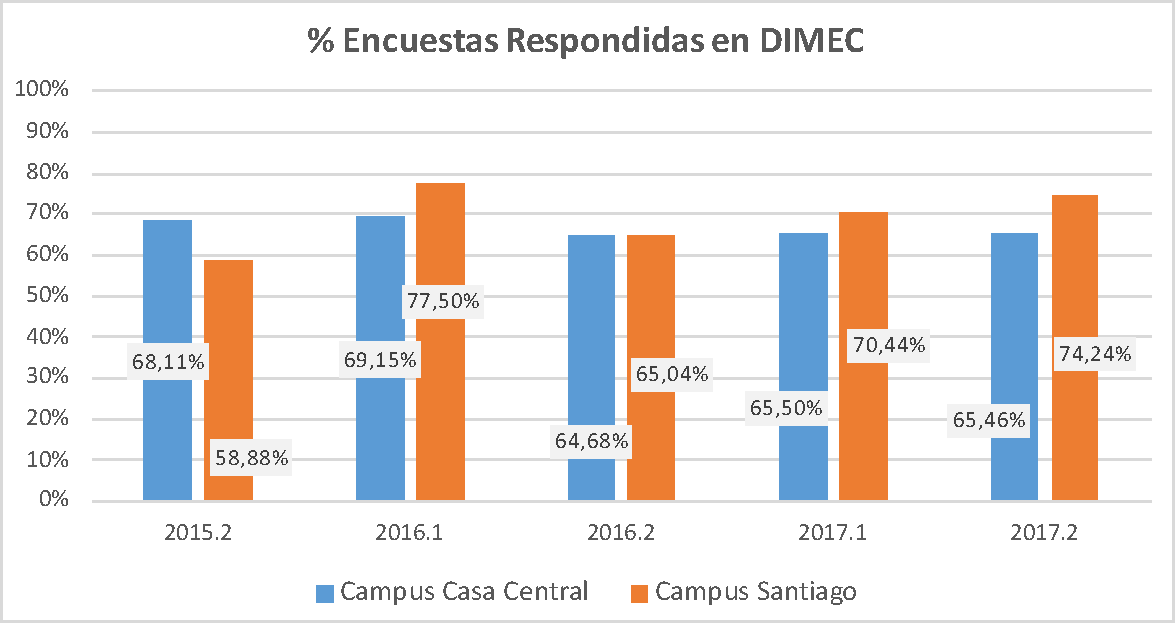
\includegraphics[width=1\textwidth]{AR1Resp.pdf}
    \caption{Porcentajes históricos de encuestas respondidas, para Campus Casa Central y Campus Santiago.}
    \label{fig:resp}
\end{figure}
\begin{text}
Como se puede ver, el porcentaje de encuestas respondidas aumento en un 3,8\% para el Campus Santiago y disminuyó un 0,04\% en el Campus Casa Central.
\end{text}
\newpage
\subsection{Análisis Comparativo del estado de aprobación del DIMEC}
\begin{text}
De la figura mostrada a continuación se puede desprender lo siguiente: En el segundo semestre del 2017 aumentó el porcentaje de aprobación de las asignaturas, en comparación tanto con el periodo anterior (2017.1) como con el semestre equivalente anterior (2016.2).\par
Más detalladamente, en el Campus Casa Central, el aumento fue de 1,65 puntos porcentuales respecto al 2016.2 (de 89,1\% a 90,75\%. En el Campus Santiago en cambio, el aumento fue de 0,64 puntos porcentuales (de 90,41\% a 91,05\%).\par
La brecha de aprobación entre Campus Santiago y Campus Casa Central disminuyo a 0,3 puntos porcentuales a favor del Campus Santiago, y en comparación con el semestre equivalente (2016.2) esto se debe mayormente al aumento de un 1,65\% en la aprobación del Campus Casa Central. \par

\end{text}
 
\begin{figure}[H]
    \centering
    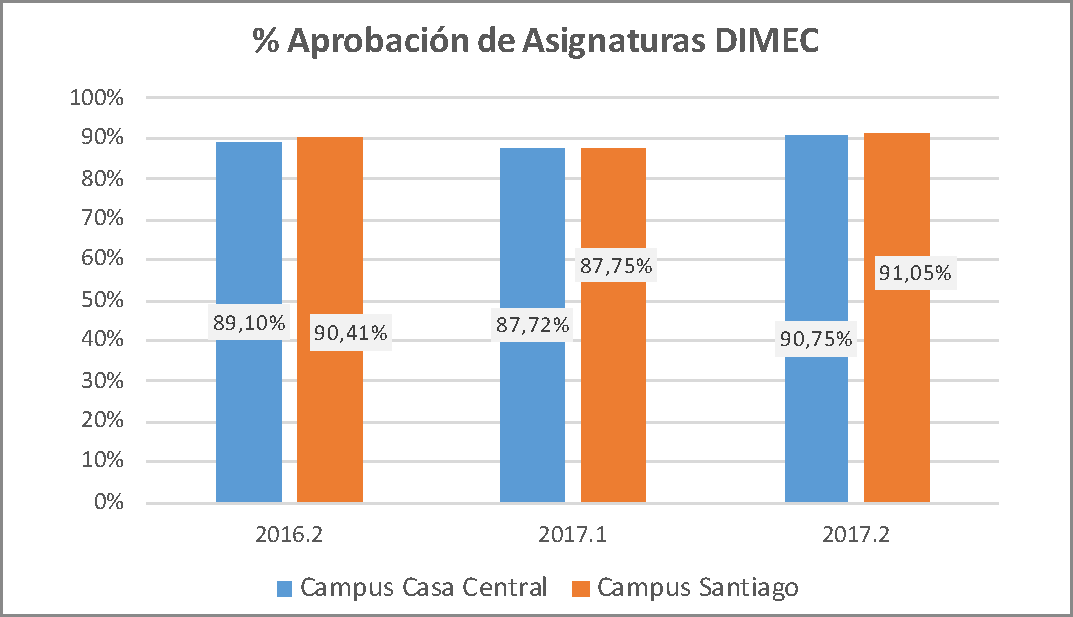
\includegraphics[width=1\textwidth]{AR2Aprob.pdf}
    \caption{Porcentaje de aprobación promedio de todas las asignaturas impartidas por el DIMEC, periodos 2016.2, 2017.1 y 2017.2.}
    \label{fig:resp}
\end{figure}
\newpage
\subsection{Análisis Comparativo de los resultados obtenidos del DIMEC entre Campus}

En relación a los puntajes obtenidos en la encuesta docente, en los ítems de importancia para el DIMEC, se tienen los siguientes resultados: 
\begin{figure}[H]
    \centering
    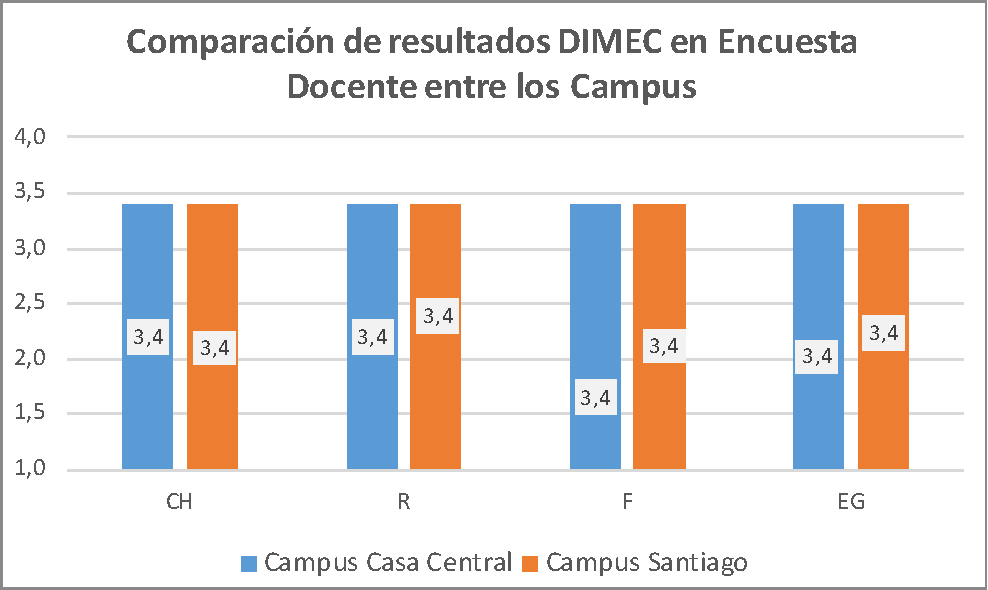
\includegraphics[width=1\textwidth]{AR3Resultados.pdf}
    \caption{Resultado promedio para cada ítem evaluado en la encuesta docente del 2017.2.}
    \label{fig:resp}
\end{figure}

De lo que se desprende que:
\begin{itemize}
    \item Los resultados son equivalentes entre ambos Campus para cada uno de los ítems evaluados: Manejo de Contenido y Habilidades Pedagógicas (CH), Relación Profesor/Estudiante (R), Aspectos Formales (F) y Evaluación Global (EG).
    \item En la perspectiva de comparación con el semestre equivalente anterior (2016.2), se muestra una disminución en las calificaciones de todos los indicadores medidos. \\ En el caso de los ítems de Manejo del Contenido y Habilidades Pedagógicas (CH) y de Relación Profesor/Estudiante (R) la disminución fue de 0,1 puntos, pasando de haber obtenido 3,5 en 2016.2 a 3,4 de calificación, estos datos coincidieron entre ambos campus. \\ Así mismo, las calificaciones de los factores de Evaluación Global (EG) y Aspectos Formales (F) coincidieron también entre los Campus, registrando una de 0,2 puntos (de 3,6 en 2016.2 a 3,4).\\ En conclusión, la evaluación del DIMEC en su conjunto muestra una merma de entre 3\% y 5\% con respecto al periodo equivalente anterior (2016.2), aun así, los resultados no dejan de considerarse positivos. 
    \item Se destaca que, dados los gráficos mostrados en la sección 3.2 donde se visualizan los rangos extremos obtenidos en cada ítem, se puede concluir que en el DIMEC en conjunto (considerando ambos campus) una muy pequeña cantidad de paralelos evaluó a su profesor con un promedio menor a 2,5 puntos en todas las categorías. Es por esto que los gráficos de Rangos Inferiores son muy pequeños. 
\end{itemize}

\subsection{Observaciones y recomendaciones sobre la Evaluación Docente correspondiente al segundo semestre 2016}

\begin{text}
Considerando el desempeño docente del DIMEC durante el periodo en estudio, y buscando disminuir las diferencias entre ambos campus y entre DIMEC con su respectivo campus se recomienda:

\begin{enumerate}
    \item Para mejorar la estandarización de la calidad de la docencia en ambos campus: \\                 \begin{itemize}
            \item Mejorar la coordinación efectuada en las asignaturas similares impartidas en ambos campus, para homogeneizar las condiciones en que se imparten y evalúan. 
            \item Evaluar la relación que pueda existir entre las evaluaciones en la encuesta docente y factores como Prioridad Académica y la Calificación; principalmente en las asignaturas que presentan las mayores diferencias en las calificaciones entre los distintos paralelos. 
            \item Evaluar en una sesión del Consejo del DIMEC, las diferencias en evaluación producidas entre el Campus Santiago y el Campus Casa Central. 
        \end{itemize}
    \item Evaluar la labor de los docentes que han sido calificados de manera deficiente, en varios ítems en los últimos tres períodos, especialmente en los  relevantes para el DIMEC; analizar las causas de la mala evaluación, y tomar medidas correctivas al respecto.
    \item Analizar las posibles causas de los malos resultados en los cursos con mayor reprobación y tomar medidas que permitan evitar esta situación, sin perjudicar la calidad de la docencia en el ramo; verificando la efectividad de esas medidas al final del siguiente semestre académico.
\end{enumerate} \par

Para mejorar el proceso de enseñanza-aprendizaje y la consecuente evaluación docente se recomienda en lo inmediato:

\begin{enumerate}
    \item Que los profesores que hayan sido calificados deficientes en alguno de los ítems críticos de la encuesta docente, se comprometan con lo siguiente: \\
        \begin{itemize}
            \item Implanta medidas tendientes a mejorar los aspectos negativos.
            \item Participar en los cursos, diplomados o seminarios de mejoramiento de la metodología educativas, que programe la USM o el DIMEC en los periodos académicos siguientes.
        \end{itemize}
    \item Que se verifique la continuidad y efectividad de los planes de acción previos que hayan resultado del análisis de periodos anteriores.     
\end{enumerate}
\end{text}

\newpage
\vspace*{7cm}
\centering
\begin{minipage}[c]{.45\textwidth}
    \centering
    \noindent\rule{\textwidth}{0.4pt} \\
    \textbf{Luis Guzmán Bonet} \\
    Jefe de Carrera Campus Santiago
\end{minipage}\hfill
\begin{minipage}{.45\textwidth}
    \centering
    \noindent\rule{\textwidth}{0.4pt} \\
    \textbf{Guillermo González Baquedano}\\
    Jefe de Carrera Campus Casa Central
\end{minipage}

\vspace*{5cm}
\begin{minipage}{.45\textwidth}
    \centering
    \noindent\rule{\textwidth}{0.4pt} \\
    \textbf{Franco Perazzo Maggi}\\
    Coordinador de Aseguramiento de la Calidad DIMEC
\end{minipage}

\end{document}
